\chapter{Applications of transmission lines}\label{lec:lec10}
This chapter deals with the applications of transmission line at high frequency. In the previous chapters, we dealt with the
analysis of transmission line that is, the derivation of transmission line equations, power flow in transmission line, voltage and wave characteristics of transmission line, the use of graphical tool called a Smith Chart to analyze the transmission line.
There are many applications of transmission line but at high frequency, many of the reactive elements are replaced by transmission line sections. This is the part we shall discuss in this chapter.
\begin{enumerate}[(i)]
\item Measurement of Unknown Impedance 
\item As a Circuit Element
\item As a Resonant Circuit
\item Step Up Transformer 
\item Matching Impedance
\end{enumerate}

\section{Measurement of unknown impedance}
The measurement of phase is a very difficult task at high frequency. Phase measurement is crucial in impedance measurement because the impedance of a circuit consists of both the resistance and the reactance, and the reactance component depends on the phase relationship between the current and the voltage in the circuit. At high frequencies, it becomes difficult to measure the phase of signals accurately due to several factors, such as signal distortion, noise, and the limited frequency response of measurement instrument. For instance, the phase shift caused by the circuit under test becomes very small at high frequencies. Additionally, the propagation delay in cables, connectors and other components used in the measurement setup becomes significant at high frequencies and can introduce errors in the phase measurement. Therefore, in order to measure complex impedances, we have to measure the complex voltage and complex current. Since the measurement of phase is not that simple, the measurement of complex impedance becomes difficult at high frequency. In transmission line, the temporal phase between the voltage and current gets translated into spatial phase in the form of standing wave pattern which means we can assume that the temporal phase between voltage and current is gotten by measuring the standing wave pattern on the transmission line. This is the method used for measuring unknown impedance at high frequency, using a special transmission line called \textbf{slotted
transmission line}\index{slotted transmission line}.
\begin{figure}[h]
\centering
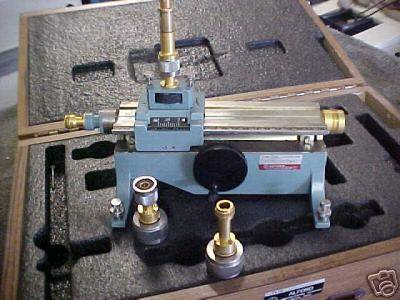
\includegraphics[width=1\linewidth]{./graphics/slottedT}
\caption{Slotted transmission line}
\label{fig:slottedT}
\end{figure}

The slotted transmission line as shown in figure~\ref{fig:slottedT} consists of a movable probe inserted in a slot in a transmission line. It determines the impedance of high-frequency circuit by using the interaction between the electromagnetic wave and the slots in the transmission line. One advantage of slotted transmission lines is that they can be used to measure the impedance of a wide range of circuits, including active and passive circuits, without the need for direct electrical contact. Additionally, slotted transmission lines can provide accurate measurements of both the magnitude and phase of the impedance, making them useful for a variety of high-frequency circuit applications. In the measurement of unknown impedance, it gives access to the transmission line in real time, to measure the voltage amplitude of the standing wave found on it. Thus by observing the standing wave (signal amplitude), one can more easily obtain the phase of the complex unknown load impedance.

The groove in the slotted transmission line is used for measuring amplitude of the voltage along the transmission line. Hence, a voltage probe slides along the transmission line, measuring the magnitude variation of the voltage from one end of the transmission line. In order to measure the unknown impedance, the voltage source has to be at one end (that is, generator end) while the load (unknown impedance) is at the load end of the transmission line as shown in figure~\ref{fig:group10diagram1}.
\begin{figure}[h]
\centering
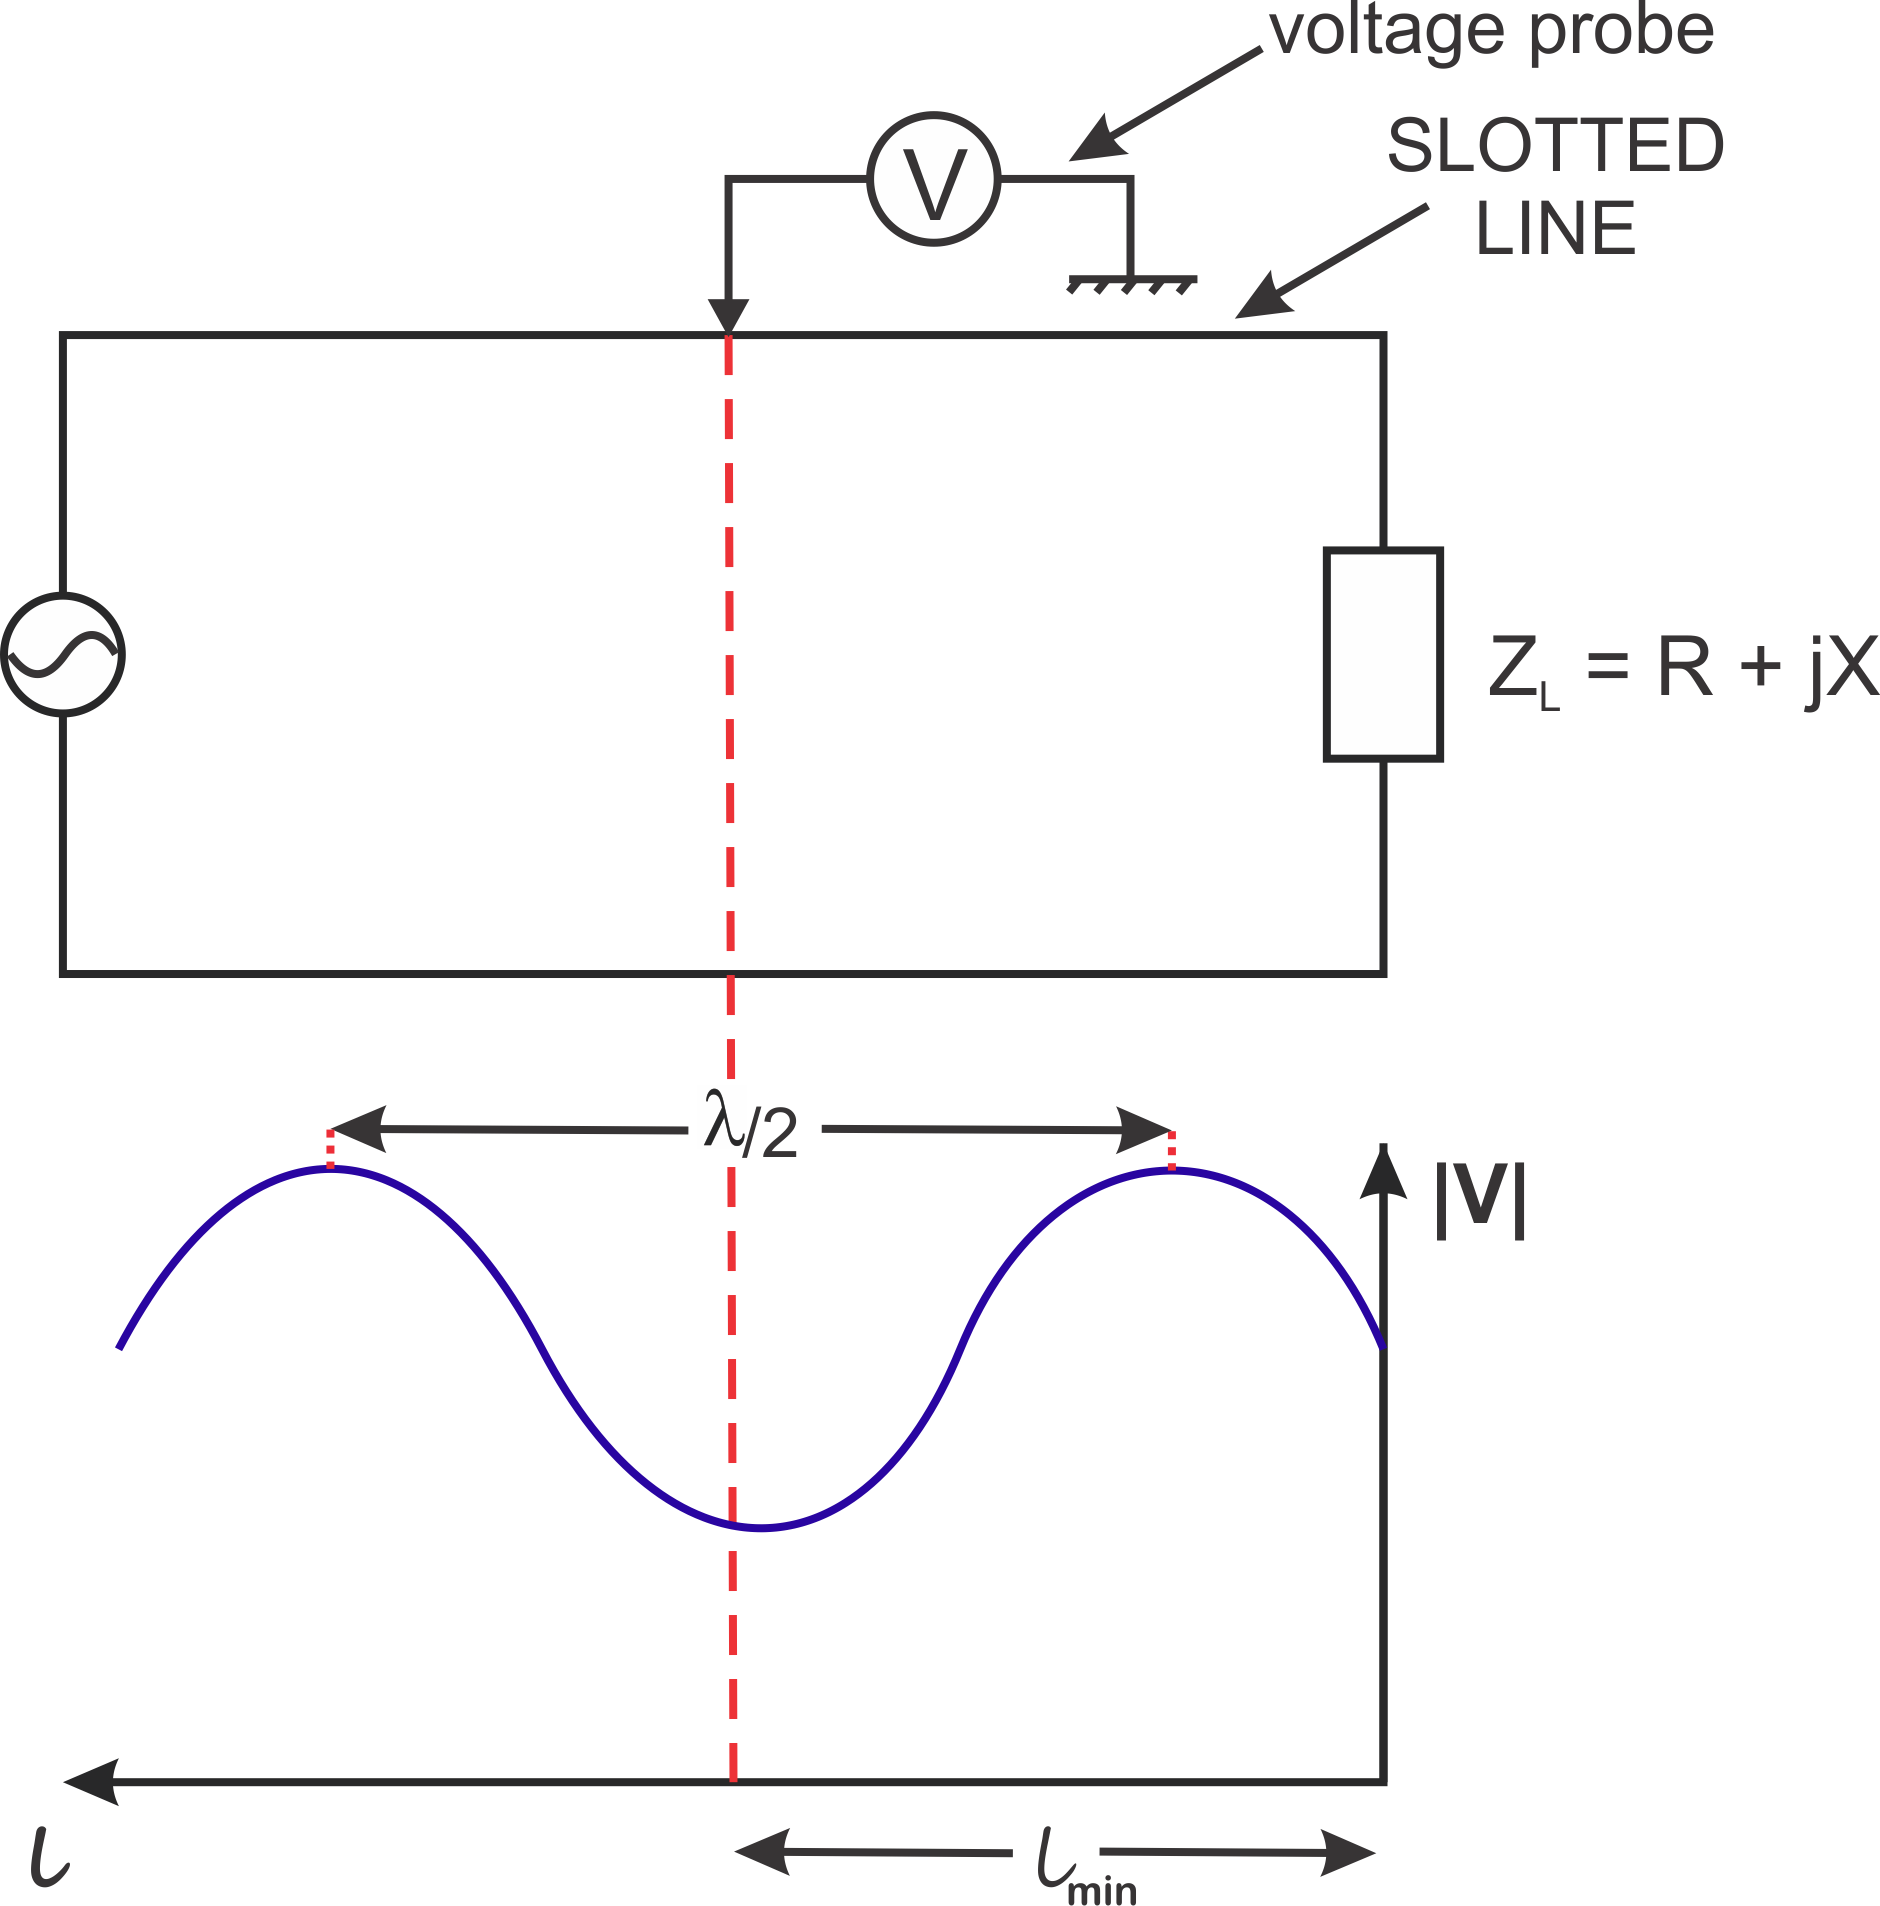
\includegraphics[width=1\linewidth]{./graphics/group10diagram1}
\caption{Measurement using the Slotted transmission line}
\label{fig:group10diagram1}
\end{figure}

The setup for the measurement is depicted in figure~\ref{fig:group10diagram1}. The unknown impedance which is to be measured is connected to the end of the tranmission line and then the tranmission line is excited with the source of desired frequency. From the standing wave patterns, the steps taken to determine the impedance are outlined as follows:
\begin{enumerate}[(i)]
\item Measure the separation between the two maxima or minima on the transmission line to estimate the value of the wavelength since the distance between two maxima or minima is $\frac{\lambda}{2}$.
\item Find the phase constant $\beta$ using $\beta = 2\frac{\pi}{\lambda}$.
\item Measure $l_\min$, which is the location of the voltage minimum from the the load end of the transmission line.
\item Measure $V_\max$ and $V_\min$ to determine the VSWR $\rho$
\item Calculate the impedance using impedance transformation relation
\end{enumerate}

\subsection{Impedance Calculation}
Recall, VSWR is given as
\begin{align}
\rho = \frac{|V|_\max}{|V|_\min}
\end{align}
Once we take measurement of $|V|_\max$ and $|V|_\min$, then we calculate for $ \rho $. We then find the maximum and minimum impedance which one can see in the transmission line. So at $l_\min$ we have $R_\min$ at that point and $R_\min$ = $\frac{Z_o}{\rho}$. Once $R_\min$ is known at $l_\min$, the calculation of unknown impedance is simply an impedance transformation problem. We recall that once the impedance at any point on the transmission line is known, the impedance at any other point can be calculated using the impedance transformation relationship.

Since we know $R_\min$ = $\frac{Z_o}{\rho}$ at $l_\min$ from the load, we can transform this impedance by a distance $l_\min$ away from the generator, so that its impedance is equal to terminating impedance $Z_{L}$. So the unknown impedance is nothing but the transformation of $R_\min$ = $\frac{Z_o}{\rho}$ by $l_\min$ to the load side of the generator. Equation~\eqref{eqn:lmintransform} is the impedance transformation relation with $l$ substituted with $l_\min$.
\begin{align}
Z_{L} = Z_o\frac{R_\min\cos(-\beta l_\min) + jZ_o\sin(-\beta l_\min)}{Z_o\cos(-\beta l_\min) + jR_\min\sin(-\beta l_\min)}
\label{eqn:lmintransform}
\end{align}
$l_\min$ is negative since we are moving away from the generator. Finding $Z_\min$ is a matter of separating the real and imaginary parts, we get the value of resistance and reactance\footnote{
We are dealing with a lossless transmission line unless otherwise stated.
} as shown below.
\begin{dmath}
Z_{L} = Z_o\frac{R_\min\cos\beta l_\min - jZ_o\sin\beta l_\min}{Z_o\cos\beta l_\min - jR_\min\sin\beta l_\min}
\end{dmath}
Rationalize into proper form by multiplying the top and bottom by the conjugate of the denominator.
\begin{dmath}
Z_{L} = Z_o\left(\frac{R_\min\cos\beta l_\min - jZ_o\sin\beta l_\min}{Z_o\cos\beta l_\min - jR_\min\sin\beta l_\min}\right)\times\left(\frac{Z_o\cos\beta l_\min + jR_\min\sin\beta l_\min}{Z_o\cos\beta l_\min + jR_\min\sin\beta l_\min}\right)
= Z_o
\frac{Z_oR_\min\cos^{2}\beta l_\min + Z_oR_\min\sin^{2}\beta l_\min}{Z_o^{2}\cos^{2}\beta l_\min + R_\min^{2}\sin^{2}\beta l_\min} +j\frac{(R_\min^{2}-Z_o^{2})\cos\beta l_\min\sin\beta l_\min}{Z_o^{2}\cos^{2}\beta l_\min + R_\min^{2}\sin^{2}\beta l_\min}
\end{dmath}
Recall $ \cos^{2}(A) + \sin^{2}(A) = 1 $ and $ \frac{\sin(A)}{\cos(A)} = \tan(A) $
\begin{dmath}
Z_{L} = Z_o \times\frac{Z_o R_\min + j(R_\min^{2}-Z_o^{2})\cos\beta l_\min\sin\beta l_\min}{(Z_o^{2}\cos^{2}\beta l_\min + R_\min^{2}\sin^{2}\beta l_\min)}
\end{dmath}
Divide numerator and denominator by $\cos^{2}\beta l_\min$:
\begin{dmath*}
Z_{L} = Z_o\frac{\frac{Z_o R_\min}{\cos^{2}\beta l_\min} + \frac{j(R_\min^{2}-Z_o^{2})\cos\beta l_\min\sin\beta l_\min}{\cos^{2}\beta l_\min}}{\frac{(Z_o^{2}\cos^{2}\beta l_\min + R_\min^{2}\sin^{2}\beta l_\min)}{\cos^{2}\beta l_\min}}
\end{dmath*}
Recall $ \frac{1}{\cos(A)} = \sec(A)$
\begin{dmath*}
Z_{L} = Z_o\left\lbrace\frac{Z_o R_\min\sec^{2}\beta l_\min + j(R_\min^{2}-Z_o^{2})\tan\beta l_\min}{Z_o^{2} + R_\min^{2}\tan^{2}\beta l_\min}\right\rbrace
\end{dmath*}
But $\frac{Z_o}{R_\min} = \rho$; dividing the numerator and denominator by $R_\min^{2}$
\begin{dmath}
Z_{L} = Z_o\left\lbrace\frac{\frac{Z_o R_\min}{R_\min^{2}}\sec^{2}\beta l_\min + \frac{j(R_\min^{2}-Z_o^{2})}{{R_\min^{2}}}\tan\beta l_\min}{\frac{1}{R_\min^{2}}{(Z_o^{2} + R_\min^{2}\tan^{2}\beta l_\min)}}\right\rbrace
= Z_o \left\lbrace\frac{\rho \sec^{2}\beta l_\min + j(1-\rho^{2})\tan\beta l_\min}{\rho^{2} + \tan^{2}\beta l_\min}\right\rbrace 
= Z_o \left\lbrace \frac{\rho (1 + \tan^{2}\beta l_\min) + j(1-\rho^{2})\tan\beta l_\min}{\rho^{2} + \tan^{2}\beta l_\min}\right\rbrace
\label{eqn:slottedtnxline}
\end{dmath}
Thus, the normalized impedance to be measured is 
\begin{dmath*}
\bar{Z_{L}} = \frac{Z_{L}}{Z_o} =  \frac{\rho (1 + \tan^{2}\beta l_\min)}{\rho^{2} + \tan^{2}\beta l_\min} + \frac{j(1-\rho^{2})\tan\beta l_\min}{\rho^{2} + \tan^{2}\beta l_\min}
\end{dmath*}
Where the real part is $R = Z_o\left[\frac{\rho (1 + \tan^{2}\beta l_\min)}{\rho^{2} + \tan^{2}\beta l_\min}\right]$ and the imaginary part is $ X = Z_o\left[\frac{(1-\rho^{2})\tan\beta l_\min}{\rho^{2} + \tan^{2}\beta l_\min}\right]$.

Hence $Z_{L} = R +jX$ can easily be calculated from all parameters that we have measured viz; $|V|_\max$, $|V|_\min$, VSWR, $\rho = \frac{|V|_\max}{|V|_\min}$, $l_\min$, and $\beta$ from $\beta = 2\frac{\pi}{\lambda}$. It can be seen that we have transformed $R_\min$ to $Z_{L}$ without necessarily knowing the value of $R_\min$, as seen in equation~\eqref{eqn:slottedtnxline}, the expression for X that is, reactance and R that is, resistance, $R_\min$ is not calculated. However, in practice, when connecting the unknown impedance to the slotted line section, we use conductors as well as other forms of connectors. This means the location of the impedance is not accurately known, so measurement of $l_\min$, sometimes become inaccurate. If we know $l_\min$ precisely, then the solution is straightforward and very accurate in finding out what the unknown impedance is. If $l_\min$ is not known, there would be error in the unknown impedance.

To avoid error, we define the location of the load by replacing it with a short circuit. Carry out the measurement of the transmission line, and find out the location of $l_\min$ with the line terminated with a short circuit. Then replace the short circuit by a load and find out the new standing wave pattern with the load. So we have two standing wave patterns on our transmission line,
\begin{enumerate}[(i)]
\item With the line terminated with a short circuit and 
\item With the unknown load terminating the line.
\end{enumerate}
For short circuits, we identify the exact location of minimum voltage by the standing wave, which becomes our origin for the unknown load impedance measurement of $l_\min$.

Hence the superposition of the load standing wave pattern on the short circuit standing wave is shown in figure~\ref{fig:group10diagram2}.
\begin{figure}[h]
\centering
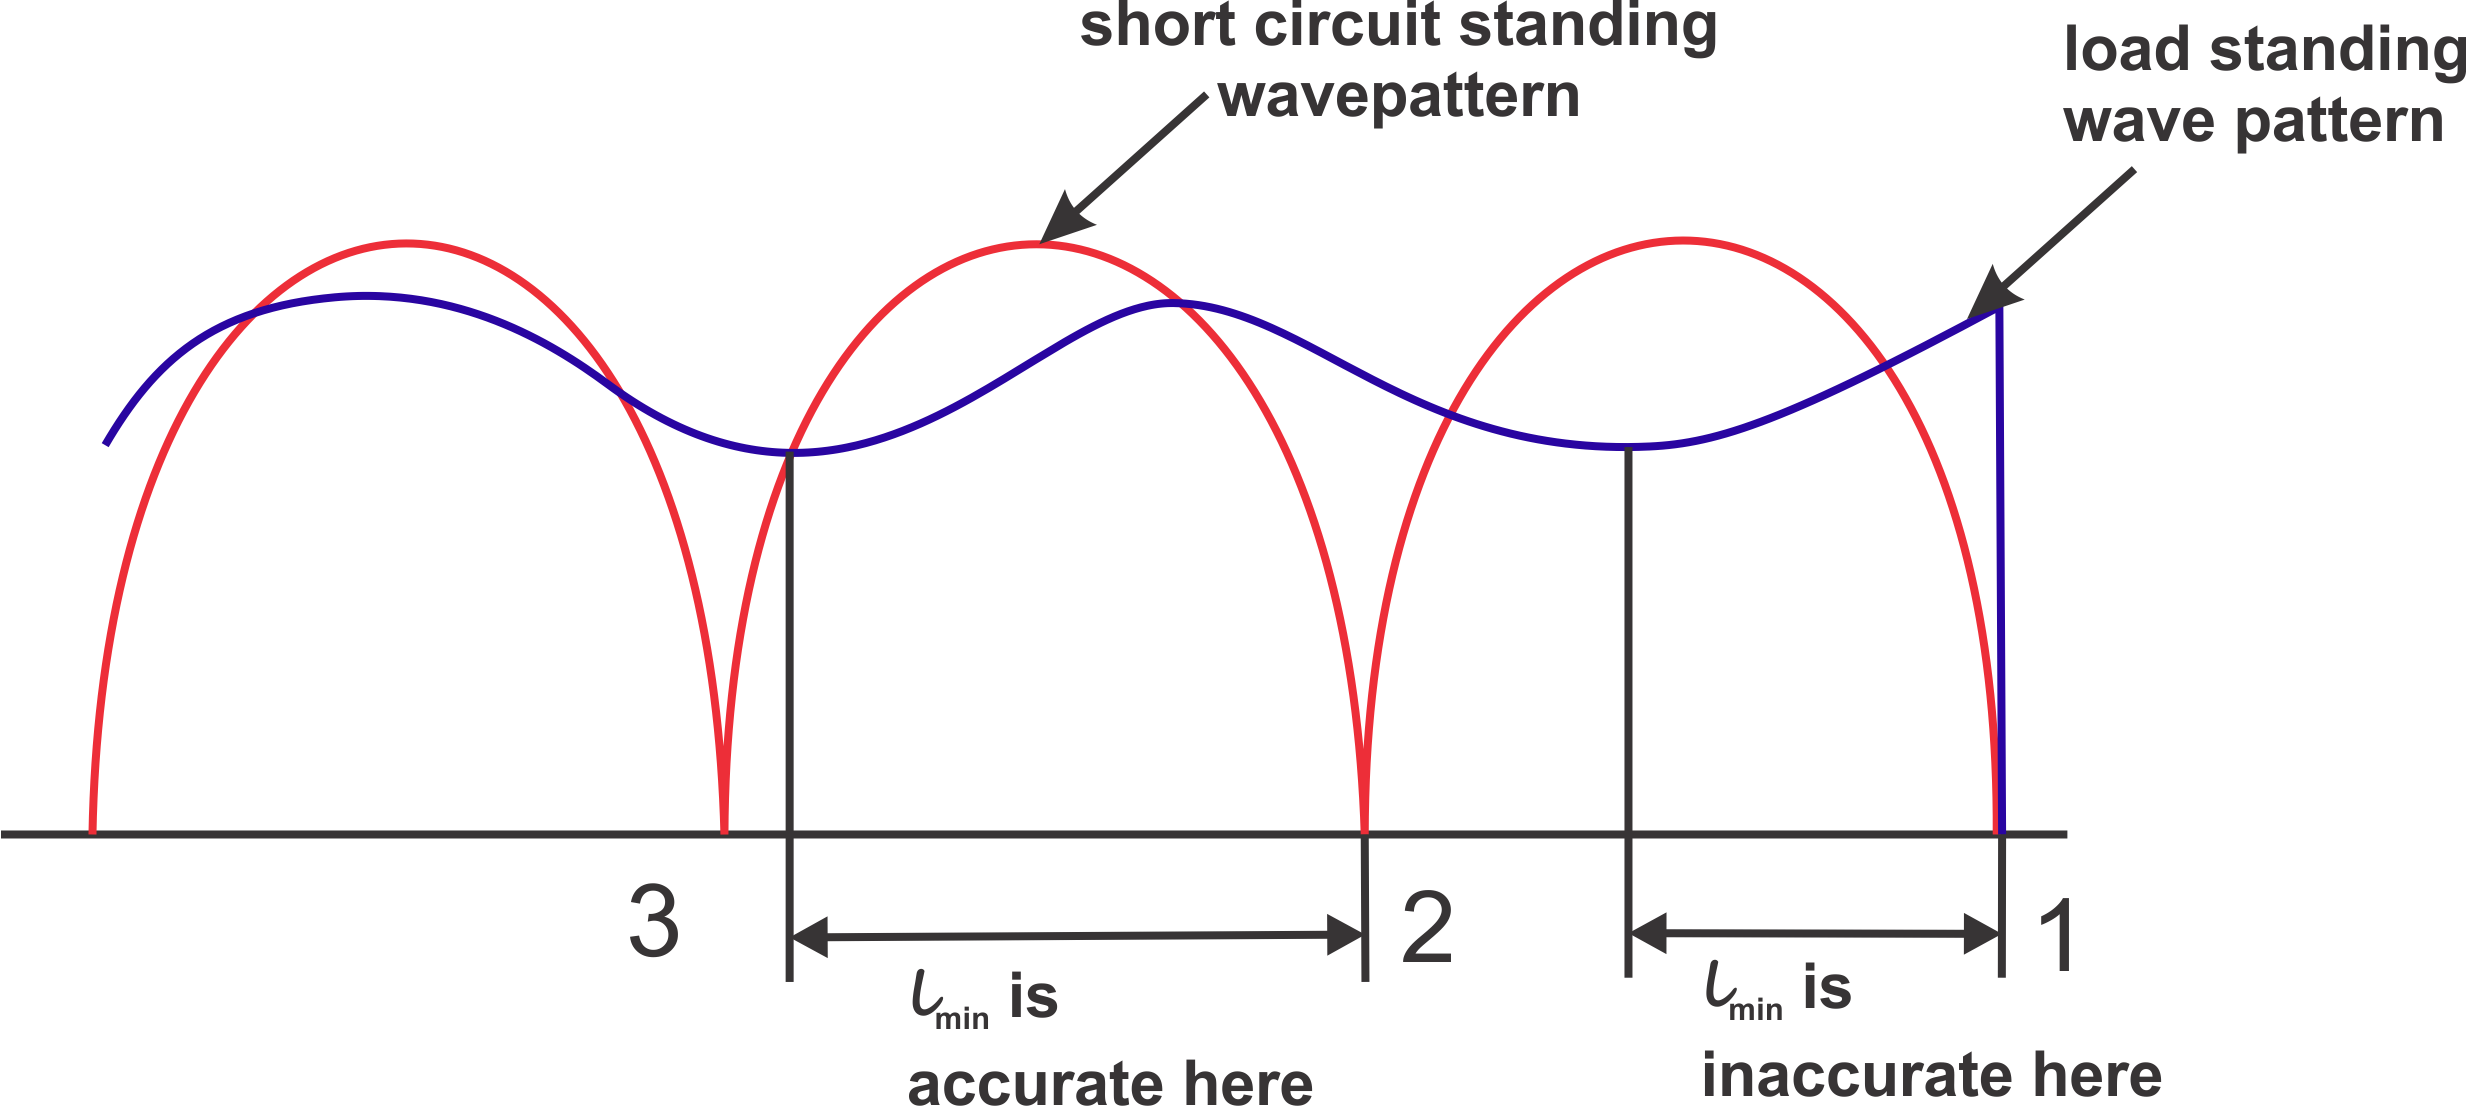
\includegraphics[width=1\linewidth]{./graphics/group10diagram2}
\caption{Superposition of the load standing wave pattern and the short circuit standing wave}
\label{fig:group10diagram2}
\end{figure}

The minimum voltage for the short circuit standing wave pattern repeats itself at $\frac{\lambda}{2}$, so we can start our measurement at position 1, 2, or 3 as shown in figure~\ref{fig:group10diagram2} and measure the corresponding distance $l_\min$ from either of these points towards the left. So instead of starting measurement at position 1 which was not accurate because of conductors used in the connection or the presence of connectors, we can start from 2 or 3 as origin and  then measure $l_\min$ of the load that occur after the first point. Thus, in practice, to find $l_\min$, we take the measurement for both short circuit and the unknown load standing wave patterns, to remove the inaccuracies introduced by the connecting conductors or connectors.

This technique of impedance measurement is very useful. In fact at high frequencies (e.g., microwave frequencies) without measurement like this on a slotted line, one will not be able to measure the unknown impedance. So at high frequency, the transmission line is suitable for the measurement of unknown impedance.

\section{As a Circuit Element}
Assuming we wound the inductor as shown in figure~\ref{fig:group10diagram3} at high frequencies such that its inductance is L. At high frequency, there is a capacitance between the turns of the inductor that almost short out current as $X_{C} = \frac{1}{2\pi f_c}$. This was not the case at low frequencies when the turns appeared separated from one another. Hence, at high frequency we then have distributed capacitors between the turns of inductor.
\begin{figure}[h]
\centering
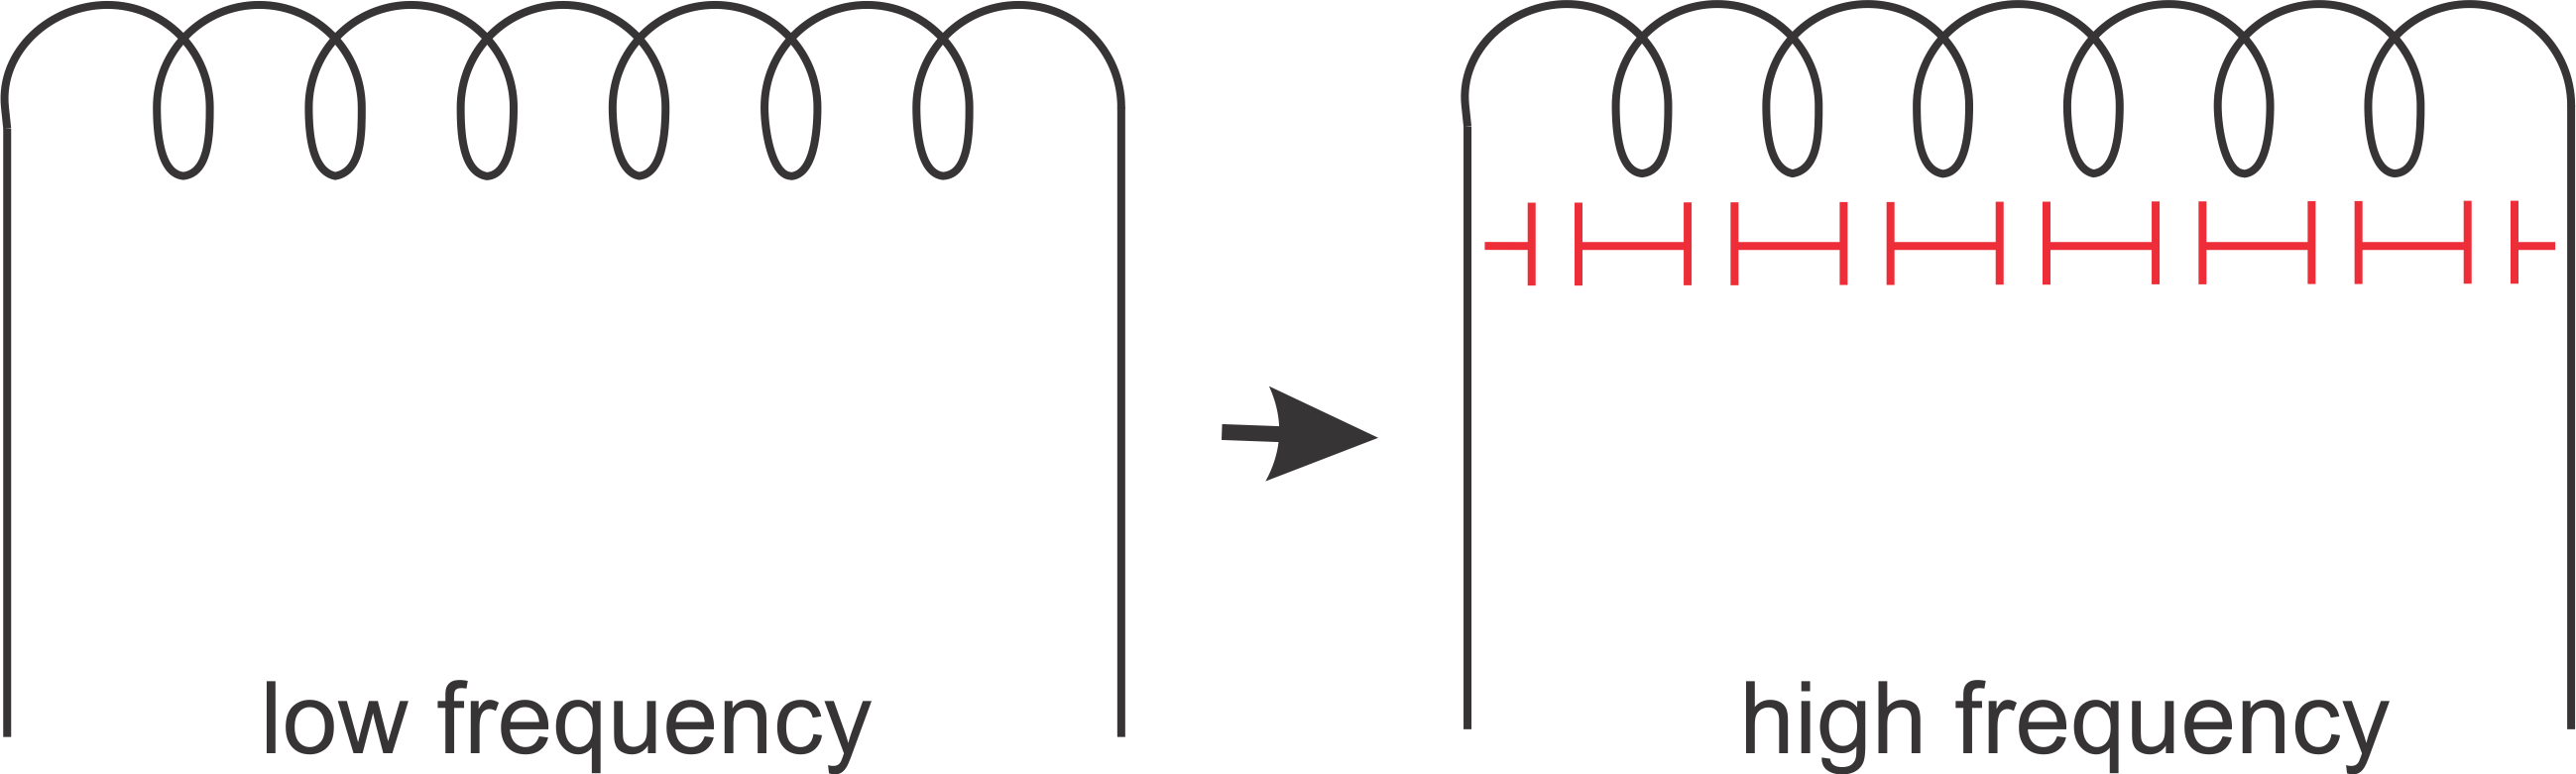
\includegraphics[width=1\linewidth]{./graphics/group10diagram3}
\caption{An inductor at Low frequency and then at High frequency}
\label{fig:group10diagram3}
\end{figure}

As the frequency increases, the inductor starts having capacitive reactance. It shows for typical wire wound inductor, the resonance frequency lies for distributed capacitances and inductances in the range of 100\textemdash\;200MHz. It means if we wound an inductor, beyond about few 100MHz, the inductor will not exhibit its ideal characteristics, but rather that of a capacitor because we have already crossed the resonance frequency. So the effect of capacitance is more dominant compared to the inductance.

Similarly, suppose we take a capacitor at low frequency, it will exhibit its ideal characteristics. As the frequency increases, the connecting leads or wires which have inductance starts to predominate beyond certain frequencies, the capacitor no longer exhibit its ideal characteristics (see figure~\ref{fig:group10diagram4}).
\begin{figure}[h]
\centering
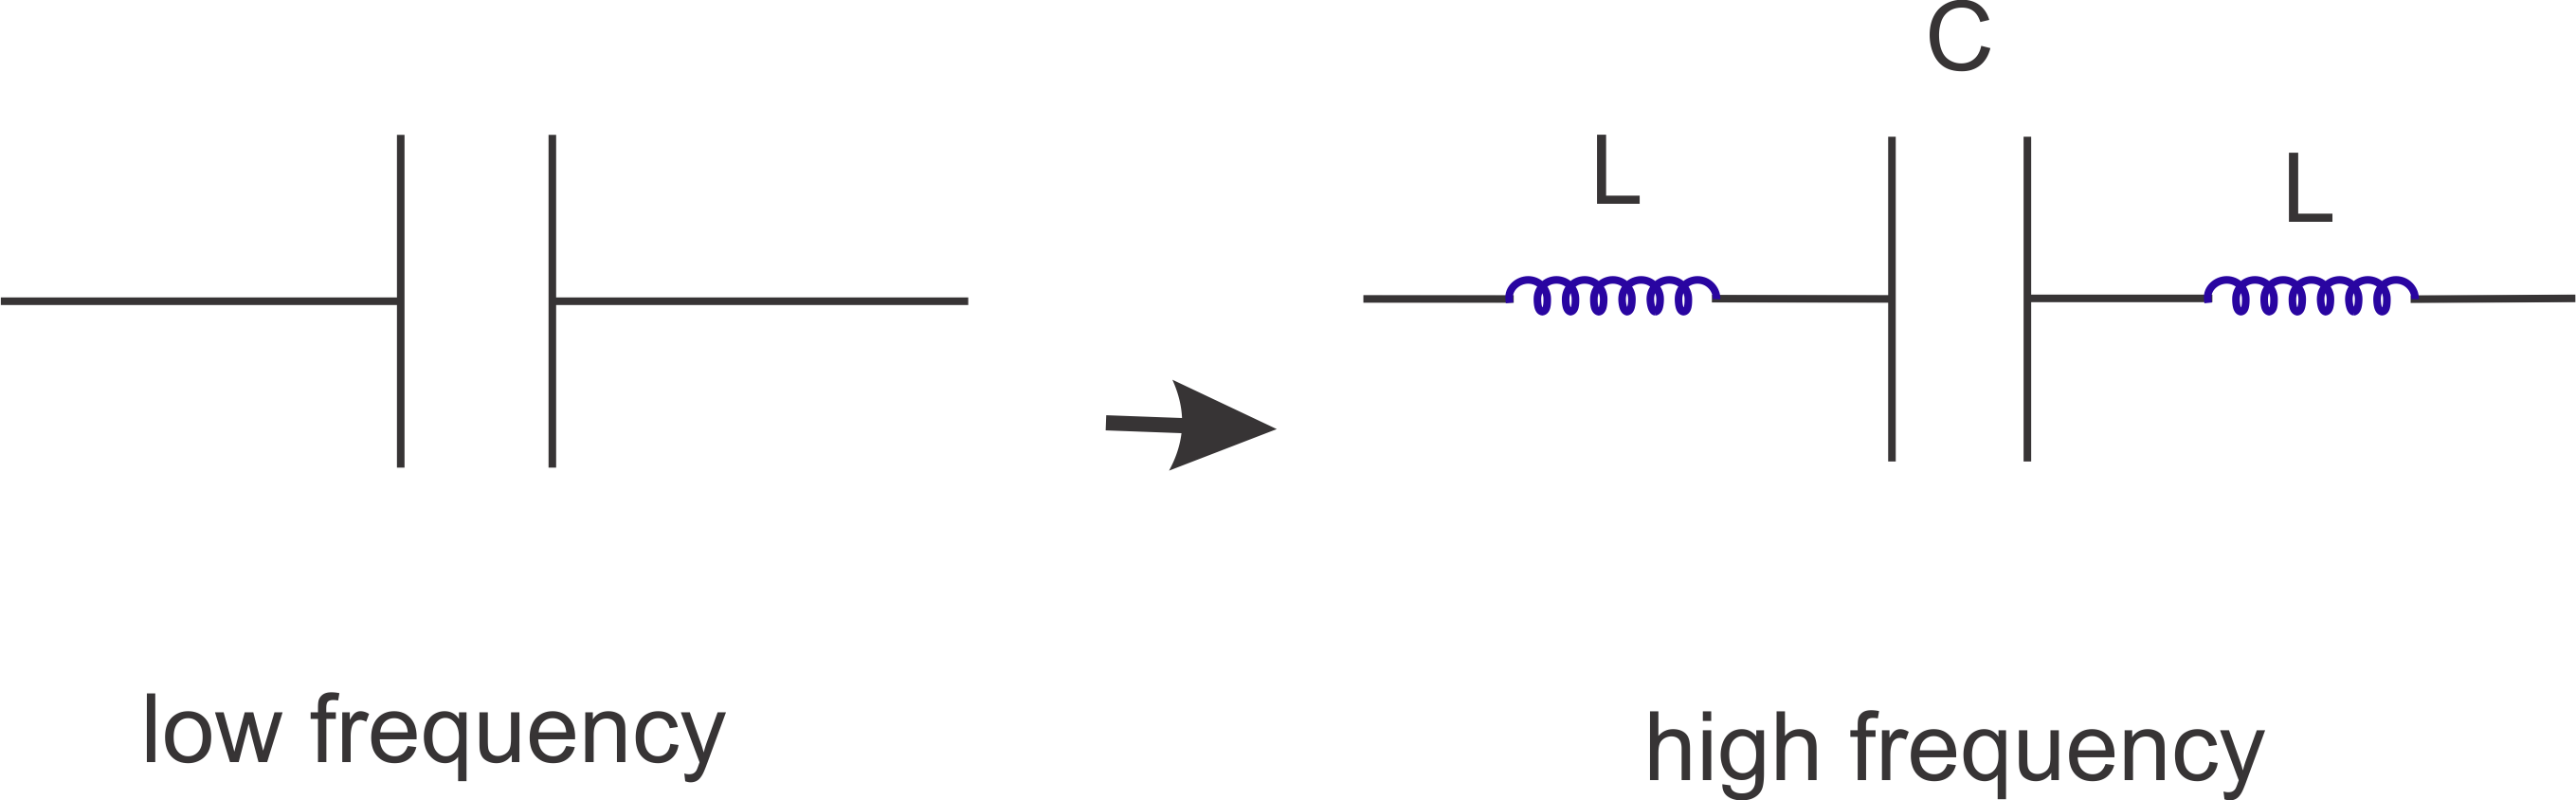
\includegraphics[width=1\linewidth]{./graphics/group10diagram4}
\caption{An capacitor at Low frequency and then at High frequency}
\label{fig:group10diagram4}
\end{figure}

Hence we can reliably design an inductor at low frequencies. But at high frequencies, its reliability is very poor because the inductor is no longer ideal. Similarly for a capacitor at high frequencies, the inductance at the leads start to predominate and the capacitor no longer exhibit its ideal characteristics. So at high frequency, realizing a reactive element is not that easy because, we do not have a reliable circuit element which will guarantee its use as a capacitor or inductor. When the frequency is increasing, the wavelength is becoming smaller as we have seen earlier. 
However, if you consider a short or open circuit transmission line, the input impedance of these lines would behave like a reactance.

So as the frequency increases and the wavelength gets smaller, the size of a transection (a small lineal element) of a transmission line which can give you impedance will be reactive; this becomes more physically realizable. Two things have become clear when working with transmission
lines and they are;
\begin{enumerate}[(i)]
\item The lumped circuits are becoming more difficult to realize at high frequency.
\item Realization of reactance by using transmission lines transection is easier, because as the wavelength becomes smaller, the transections of the transmission line becomes more feasible to realize an ideal reactive element.
\end{enumerate}
At high frequencies, most reactive transections are replaced by transmission lines as shown in figure~\ref{fig:group10diagram5}. In the impedance Smith Chart, open circuit is at the rightmost part and short circuit is at the leftmost part of the outermost circle\footnote{
The outermost circle has $r = 0$ and it implies that as we move along that circle we trace out pure reactance.
}. Moving along this outermost circle shows how much length (in terms of wavelength) is needed between load and generator to realize any pure reactance. We can assume the presence of that reactance at that point, from the open or short circuit end towards the signal source or generator.
\begin{figure}[h]
\centering
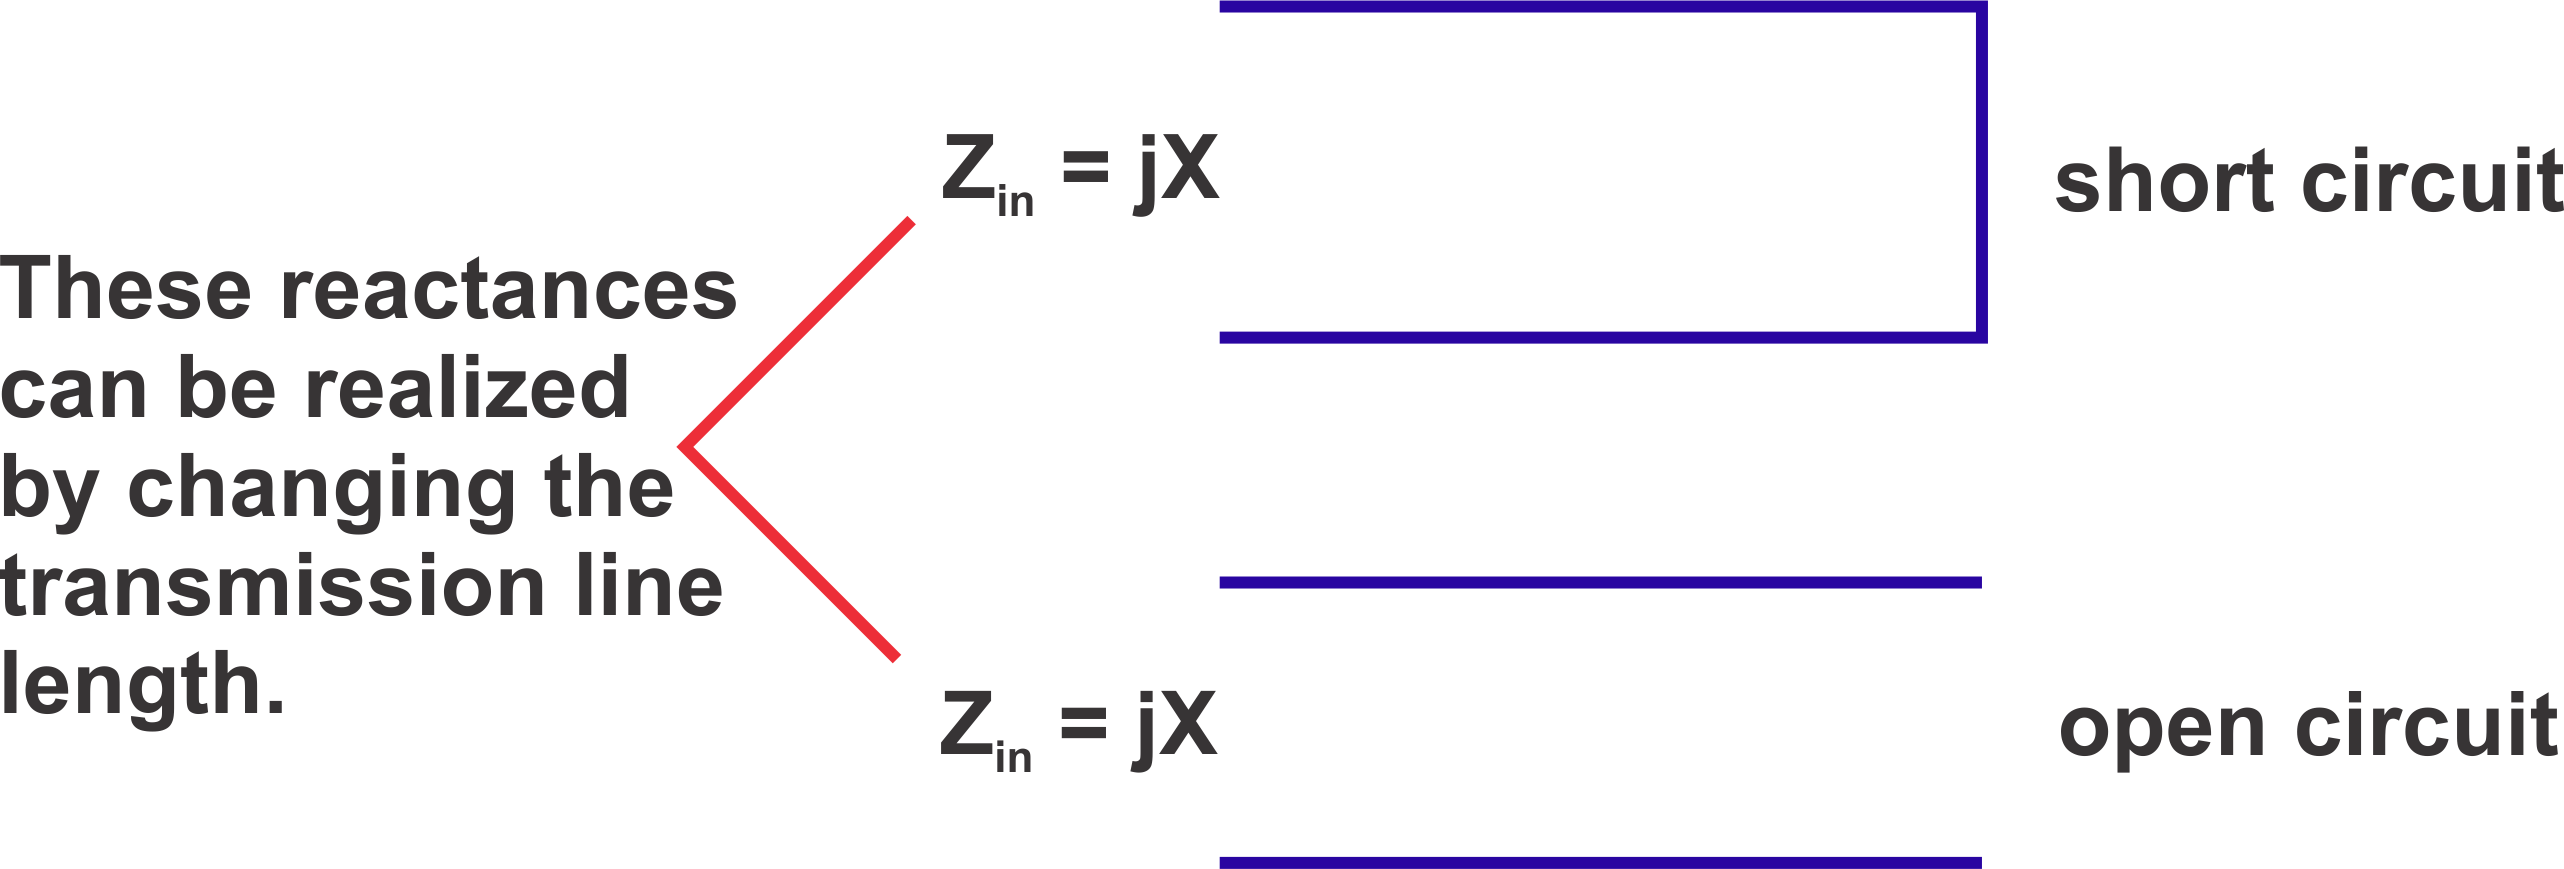
\includegraphics[width=1\linewidth]{./graphics/group10diagram5}
\caption{Transmission Line as a Circuit Element}
\label{fig:group10diagram5}
\end{figure}

Hence for a open or short circuit load, by using different length of transmission line, we can get different reactance at the input. Therefore, \emph{what should be the length of the transmission line, so that one gets a particular value of reactance at the input?}

\subsection{Analytical approach of using transmission line as a circuit element}
Analytically, $l$ is the distance towards the generator and recall that for a lossless transmission line which we assume unless stated otherwise.

Considering a short circuit load at the end of a transmission line, then using the impedance transformation relation,
\begin{dmath}
Z_{in} = Z_o \left\lbrace\frac{Z_{L}\cos\beta l + jZ_o\sin\beta l}{Z_o\cos\beta l + jZ_{L}\sin\beta l}\right\rbrace\quad Z_{L} \text{= 0 for short circuit} 
= Z_o \left\lbrace \frac{0 + jZ_o\sin\beta l}{Z_o\cos\beta l + 0}\right\rbrace  = jZ_o\tan\beta l 
\end{dmath}

Similarly, considering an open circuit load at the end of a transmission line, $Z_L = \infty$ so we take limits as $Z_L$ tends to infinity.
\begin{dmath}
Z_{in} = Z_o \left\lbrace \frac{Z_{L}\cos\beta l + jZ_o\sin\beta l}{Z_o\cos\beta l + jZ_{L}\sin\beta l}\right\rbrace \quad Z_{L} \text{= }\infty\text{ for open circuit.}
= Z_o \left\lbrace \frac{\cos\beta l + j\frac{Z_o}{Z_{L}}\sin\beta l}{\frac{Z_o}{Z_{L}}\cos\beta l + j\sin\beta l}\right\rbrace
= Z_o \left\lbrace \frac{\cos\beta l + j \times 0}{0 + j\sin\beta l}\right\rbrace = -jZ_o\cot\beta l 
\end{dmath}
Thus,
\begin{align}
Z_{in} &= jZ_o\tan\beta l \Rightarrow \text{ short circuit}\\
Z_{in} &= -jZ_o\cot\beta l \Rightarrow \text{ open circuit}
\end{align}
Hence the problem of realizing a given reactance from open or short circuit load involves finding the $l$ that gets the appropriate $Z_{in}$. 
Let $l_{SC}$ and $l_{OC}$ represent short circuit and open circuit length respectively, then we have $ X = jZ_o\tan\beta l_{sc} $ and $ X = -jZ_o\cot\beta l_{oc} $ for short circuit and open circuit respectively. Since the phase constant $ \beta $ is known for the transmission line, we make $ l_{SC} $ and $ l_{OC} $ the subject of the equations, we already know the reactance, $X$ we require, so that 
\begin{align}
l_{SC} &= \frac{1}{\beta}\tan^{-1}\frac{X}{Z_o}\\
l_{OC} &= \frac{1}{\beta}\cot^{-1}\frac{-X}{Z_o}
\end{align}

If the frequency of operation as well as velocity of the wave propagation are known, then we can find $\lambda$ and use $\beta = \frac{2\pi}{\lambda} $. Therefore, in conclusion, we can realize the unknown reactance from using transections of the transmission line. 

As we know, for such calculations as this, the use of Smith Chart comes in handy. The top half of the impedance Smith Chart at the outermost circle is pure inductance, and the bottom half is for capacitance. However, before we get into details of Smith Chart usage, we have to be sure that $X = Z_o\tan\beta l_{SC}$ and $X = -Z_o\cot\beta l_{OC}$ for all variation of $\beta l_{SC}$  from 0 to $ 2\pi $, either $\tan\beta l_{SC}$ or $\cot\beta l_{OC}$ varies from $-\infty$ to $+\infty$. Essentially, we want to measure the values of $X$ as we change the values of $l_{SC}$ or $l_{OC}$ in the transmission line, then we can realize any arbitrary value of the reactance. There is no limit to this. So any value of reactance between $-\infty$ to $+\infty$ can be realized either by short circuited line or open circuited line.

The choice of whether to use a short circuit or open circuit line will depend upon the system you want to employ the circuit element. For example supposing we have a parallel wire transmission line, then connecting the two ends of the transmission line is rather easy, as we can short the end of the transmission line. However, a transmission line like a Printed Circuit Board (PCB), with ground plane on one side and the line on top separated by a dielectric. To short circuit the line, we will have to drill a plated-through hole (or a signal-carrying conductive via) into the PCB and requires a lot of precision, so realizing a short circuit line on that configuration is rather difficult. For this reason, an open circuit line is preferred. There may be situations where the short circuit line will be preferred over the open circuit line and vice versa. Irrespective of the one used, we will be able to realize all the reactances from  $ -\infty$ to $+\infty $, that is, we can realize any capacitive or inductive reactance by using an open circuited or short circuit section of a transmission line.

\subsection{Graphical approach of using transmission line as a circuit element}
Graphically, we we want to find the length, the problem turn out to be the opposite of the impedance calculation. Since we know the input impedance $Z_{in}$ at generator end  and we know terminating impedance, $Z_{L}$ at the end of the transmission line to be 0 or $\infty$ (that is, it is short circuit or open circuit point). So the challenge is that we want to find $ l_{SC} $ or $ l_{OC} $ where the impedances are known at both ends are known.

The steps taken on the Smith Chart as outlined as follows:
\begin{enumerate}[(i)]
\item Mark the normalized impedance $\bar{Z}_{in}$ position, $\bar{Z}_{in} = jx$
\item Mark the point for a short circuit or open circuit, $jx = 0$ or $jx = \infty$ (see figure~\ref{fig:group10diagram6}).
\begin{figure}[h]
\centering
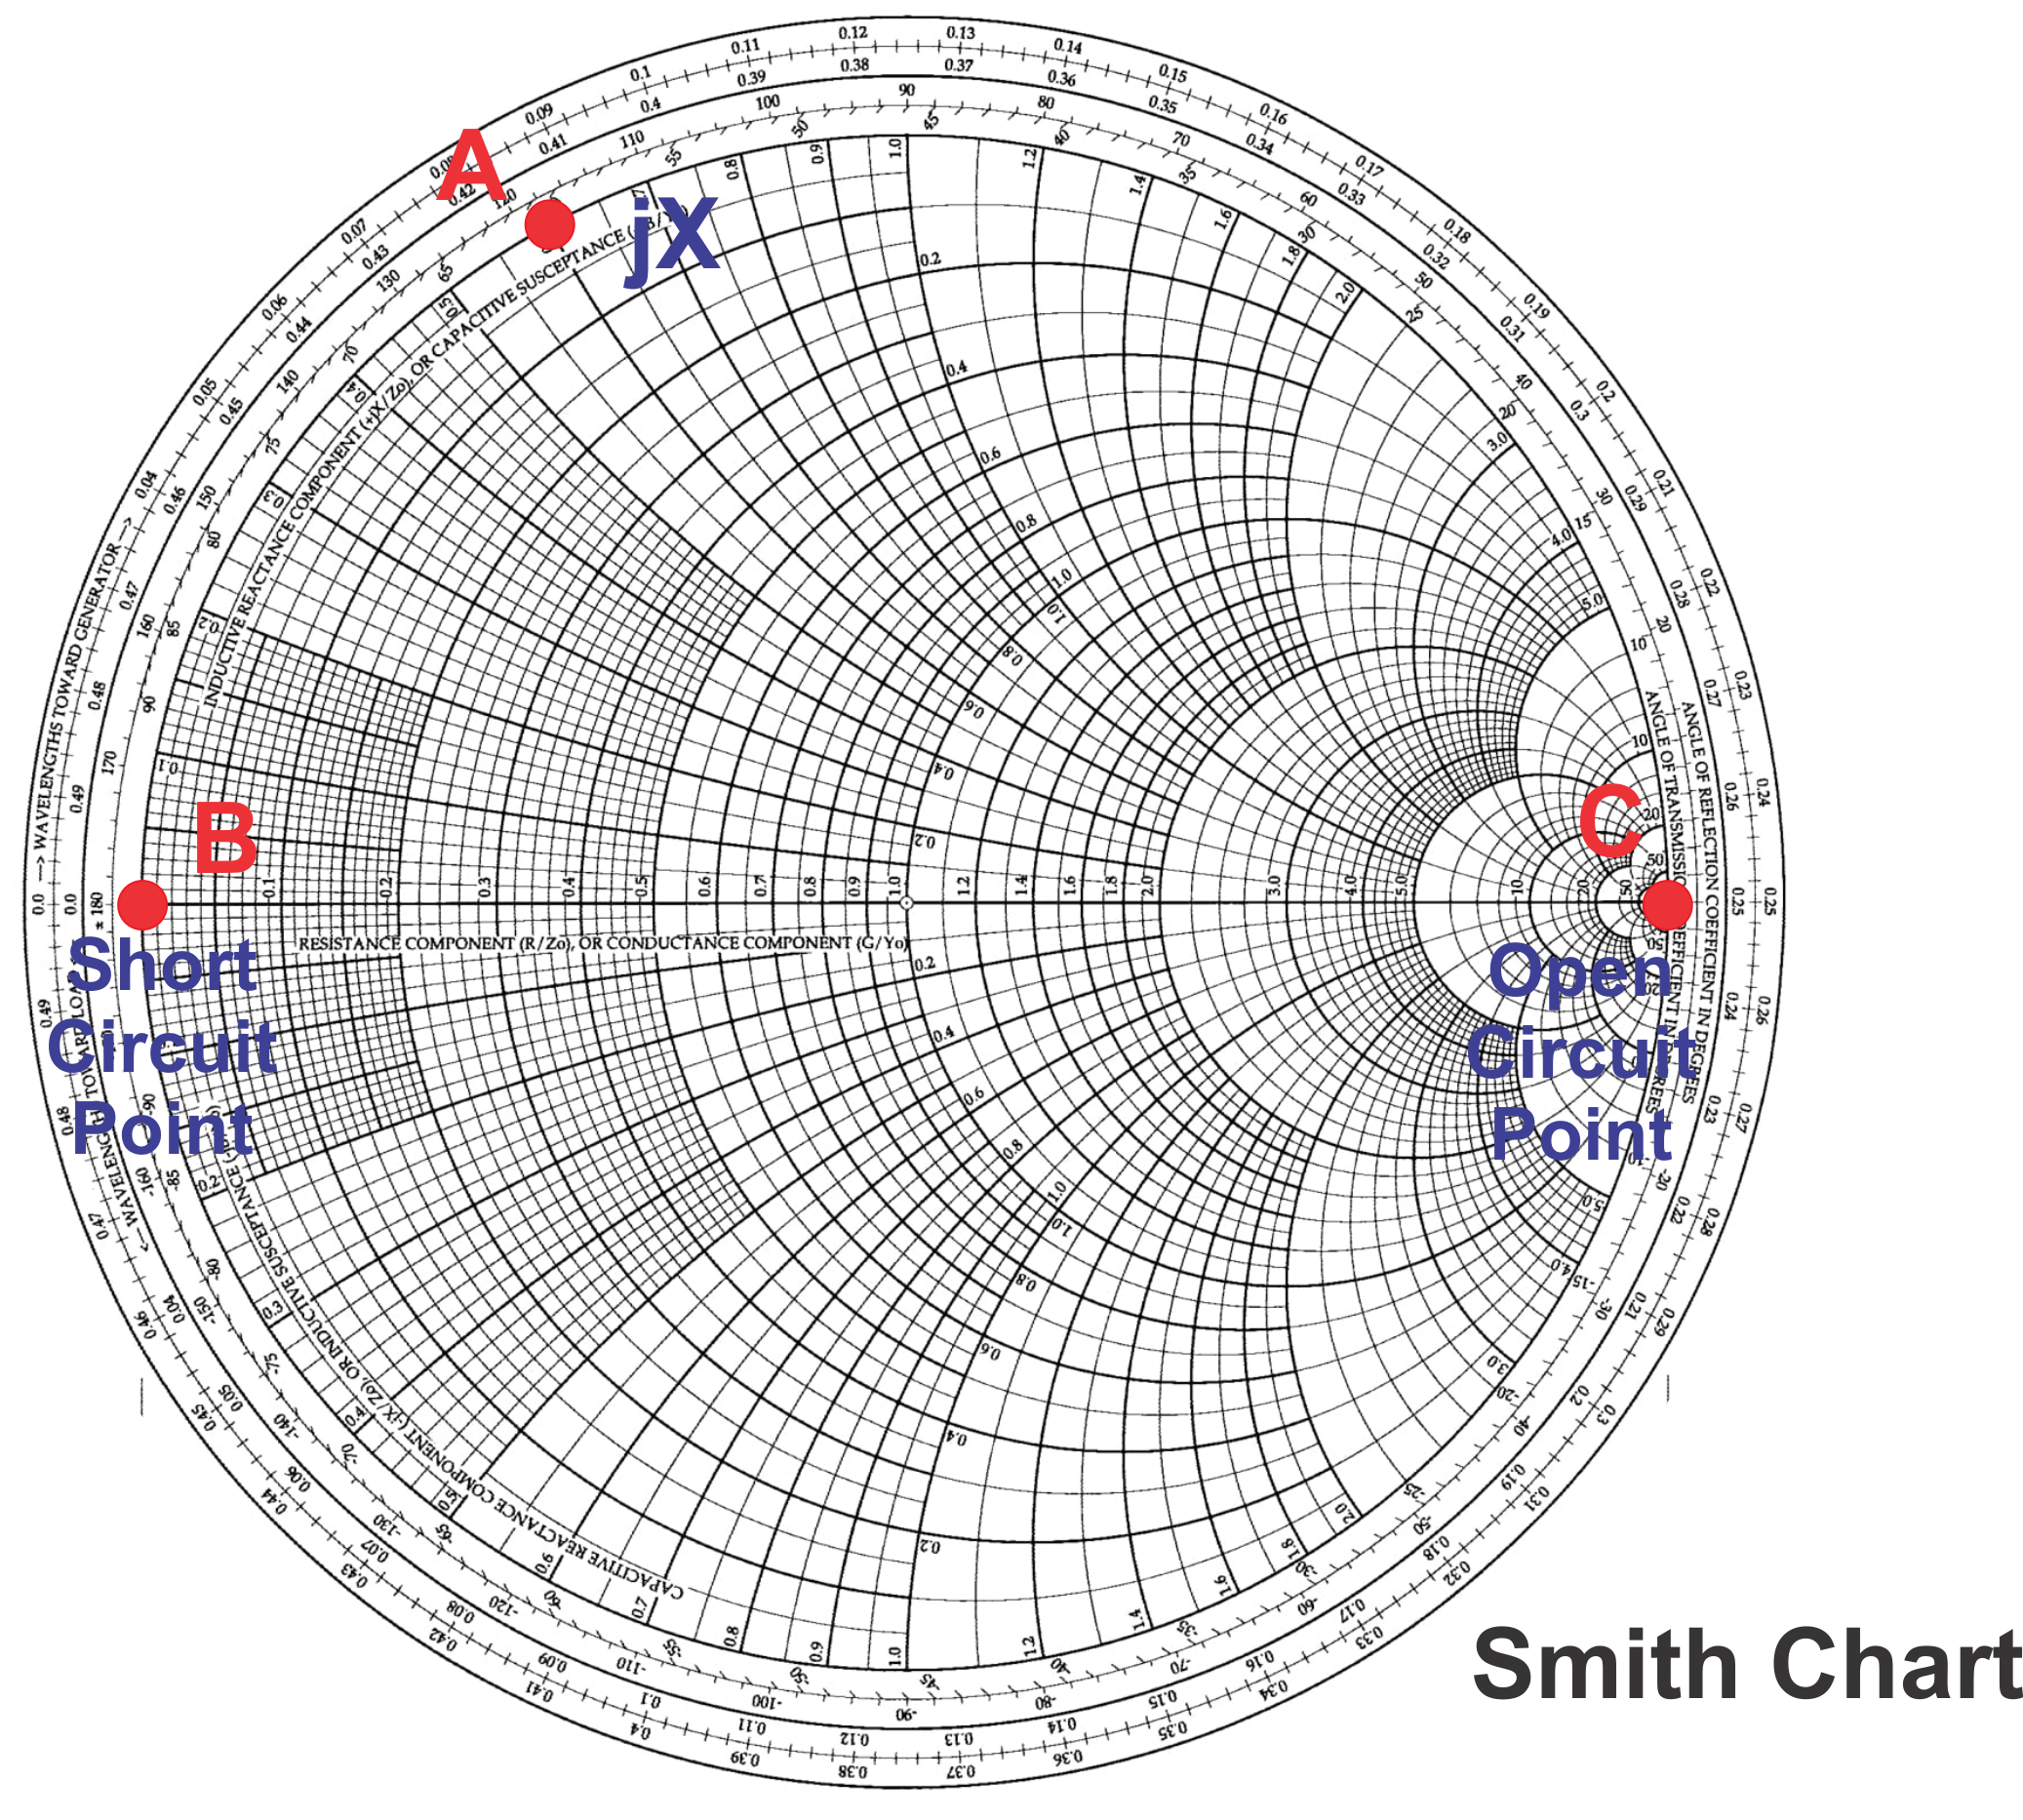
\includegraphics[width=1\linewidth]{./graphics/group10diagram6}
\caption{Open and Short Circuit points on the Smith Chart}
\label{fig:group10diagram6}
\end{figure}

\item Measure the distance from the normalized impedance $\bar{Z}_{in}$ to the short or open circuit moving counter clockwise. 
\end{enumerate}

Figure~\ref{fig:group10diagram7} shows the distances between the normalized impedance $\bar{Z}_{in}$ and the short circuit end and open circuit end respectively for an inductive reactance. Essentially we move away from the generator to reach the short circuit point, that we move from point, \textbf{A}, till we reach, \textbf{B}. On the Smith Chart, clockwise movement is towards the generator and anticlockwise movement is away from the generator.
\begin{figure}[h]
\centering
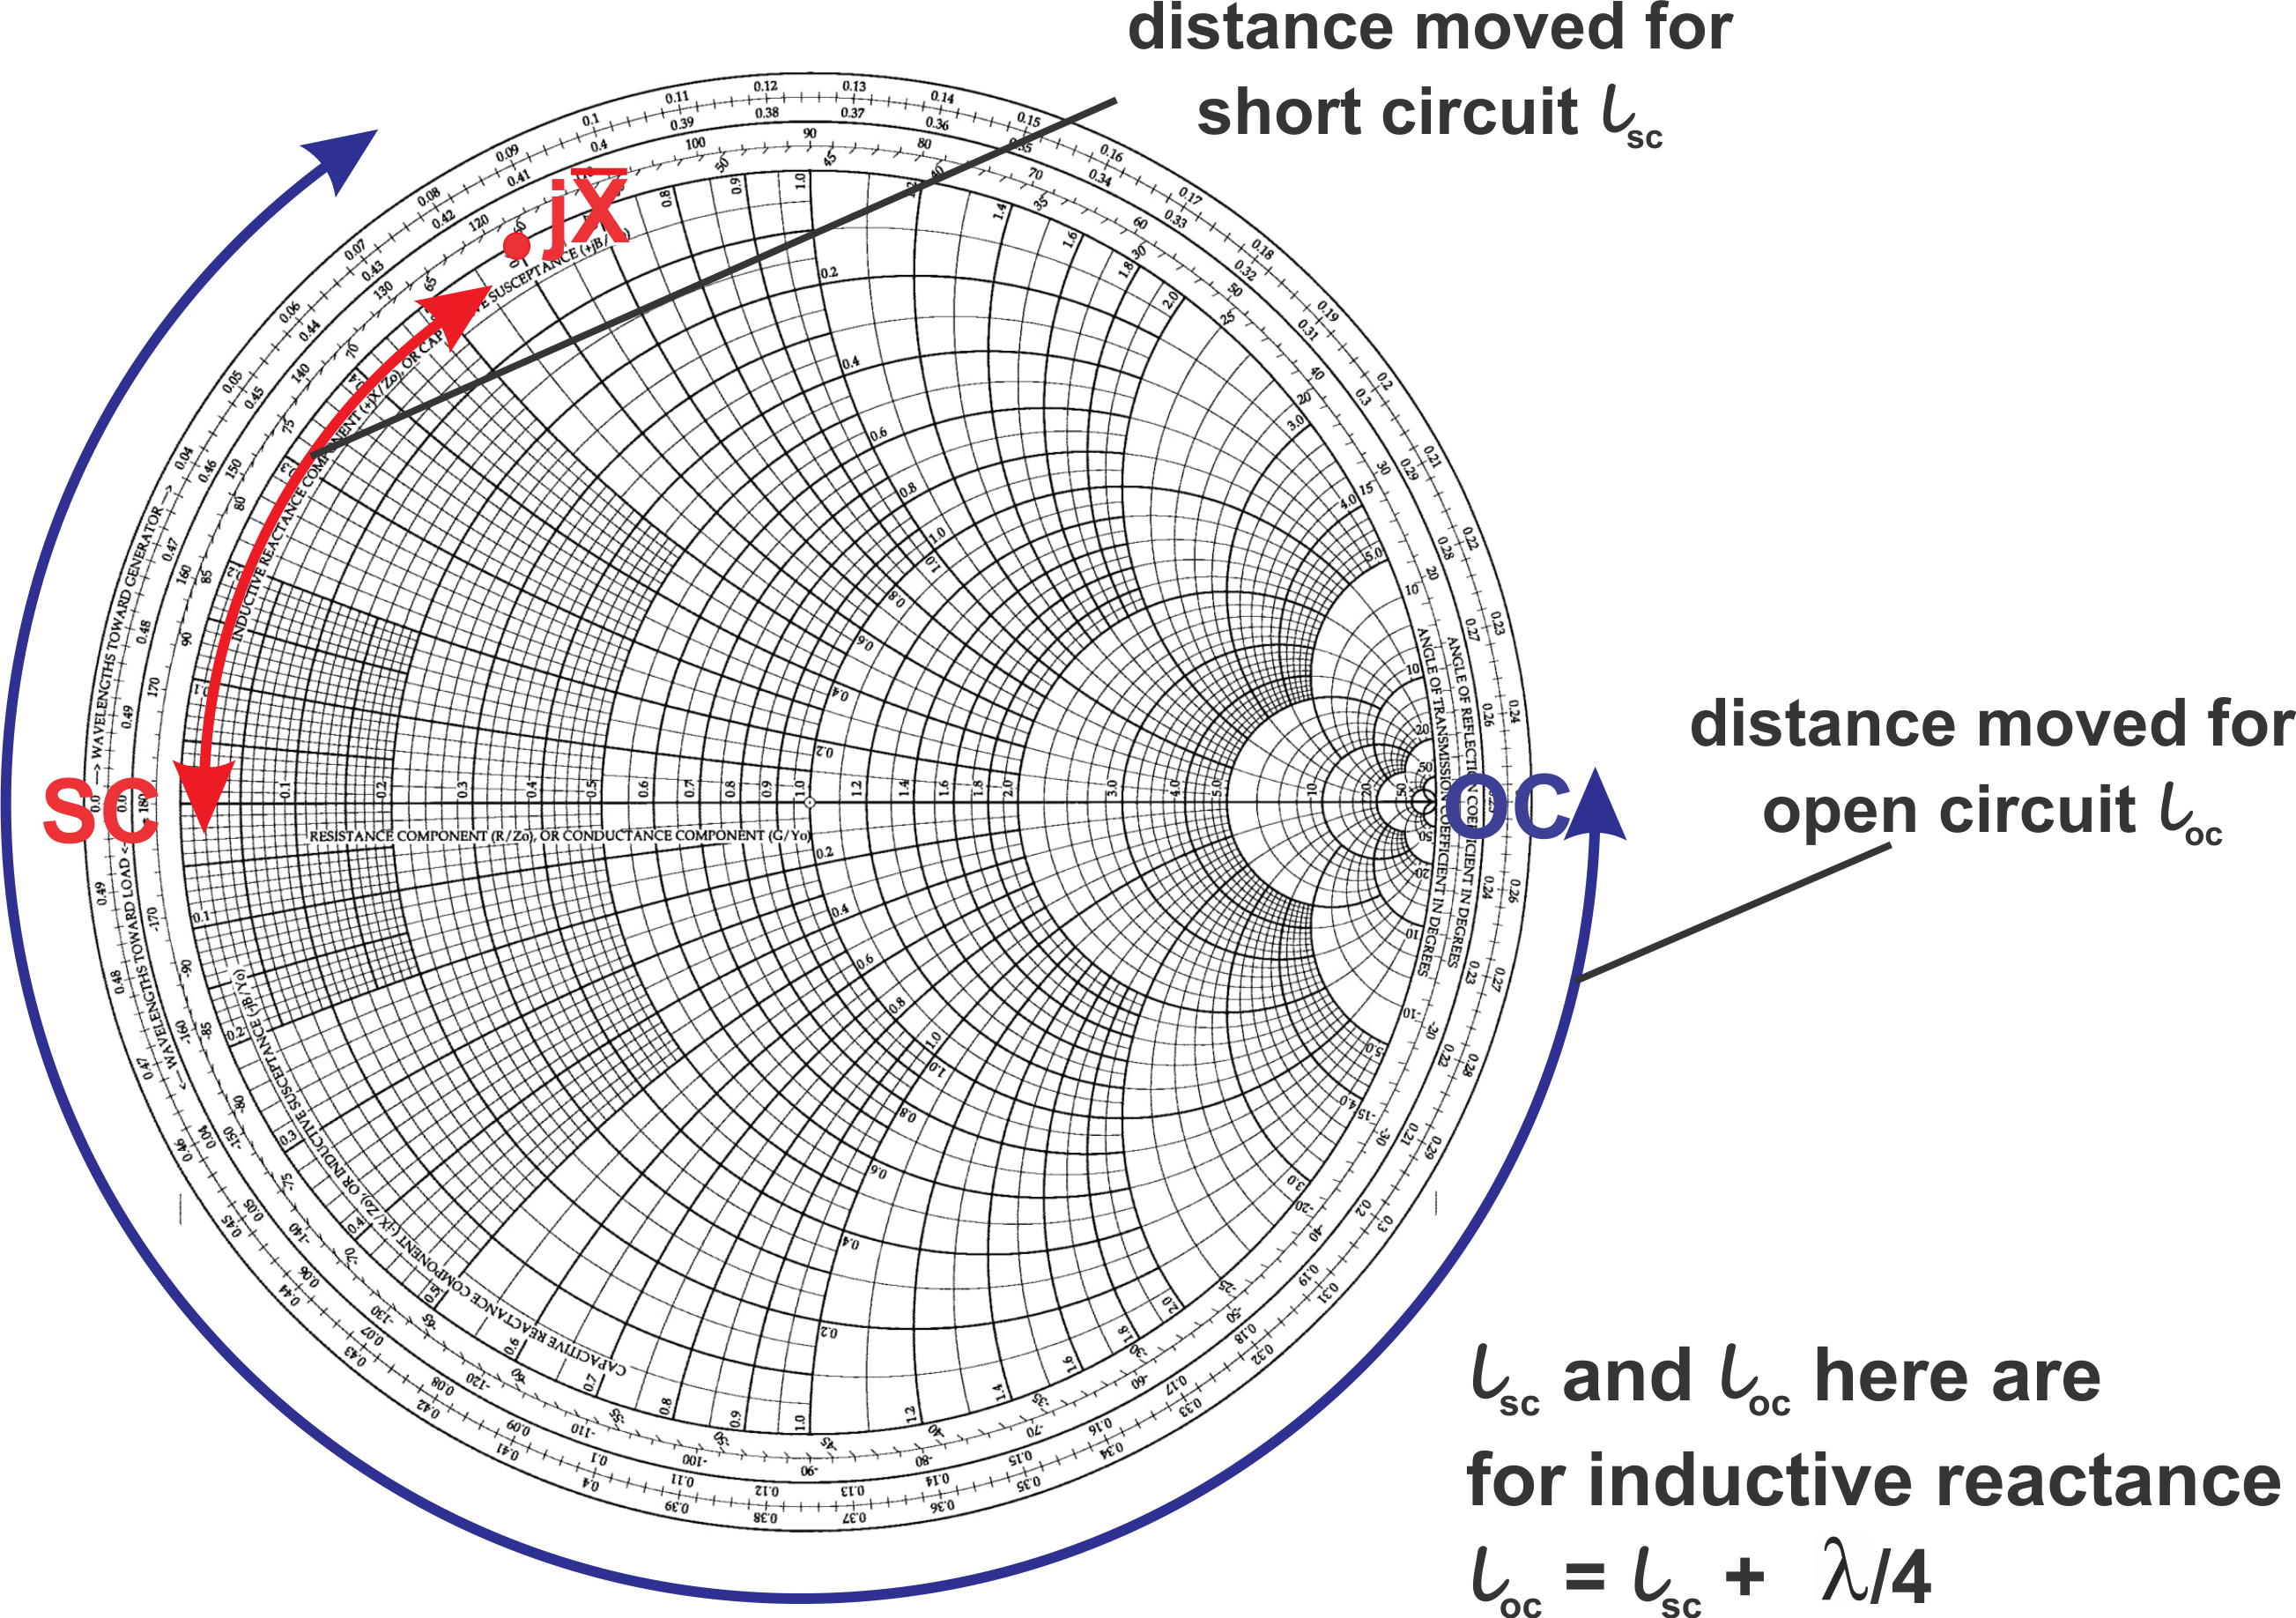
\includegraphics[scale=0.4]{./graphics/group10diagram7}
\caption{$ l_{SC} $ and $ l_{OC} $ for inductive reactance on the Smith Chart.}
\label{fig:group10diagram7}
\end{figure}

Similarly, to realize a capacitive reactance which will be located at the bottom half of the Smith Chart for a start. Moving clockwise from short circuit point by no more than $\frac{\lambda}{4}$ we have inductive reactance, but beyond that point from $\frac{\lambda}{4}$ to $\frac{\lambda}{2}$ we have capacitive reactance (see figure~\ref{fig:group10diagram9}).
\begin{figure}[h]
\centering
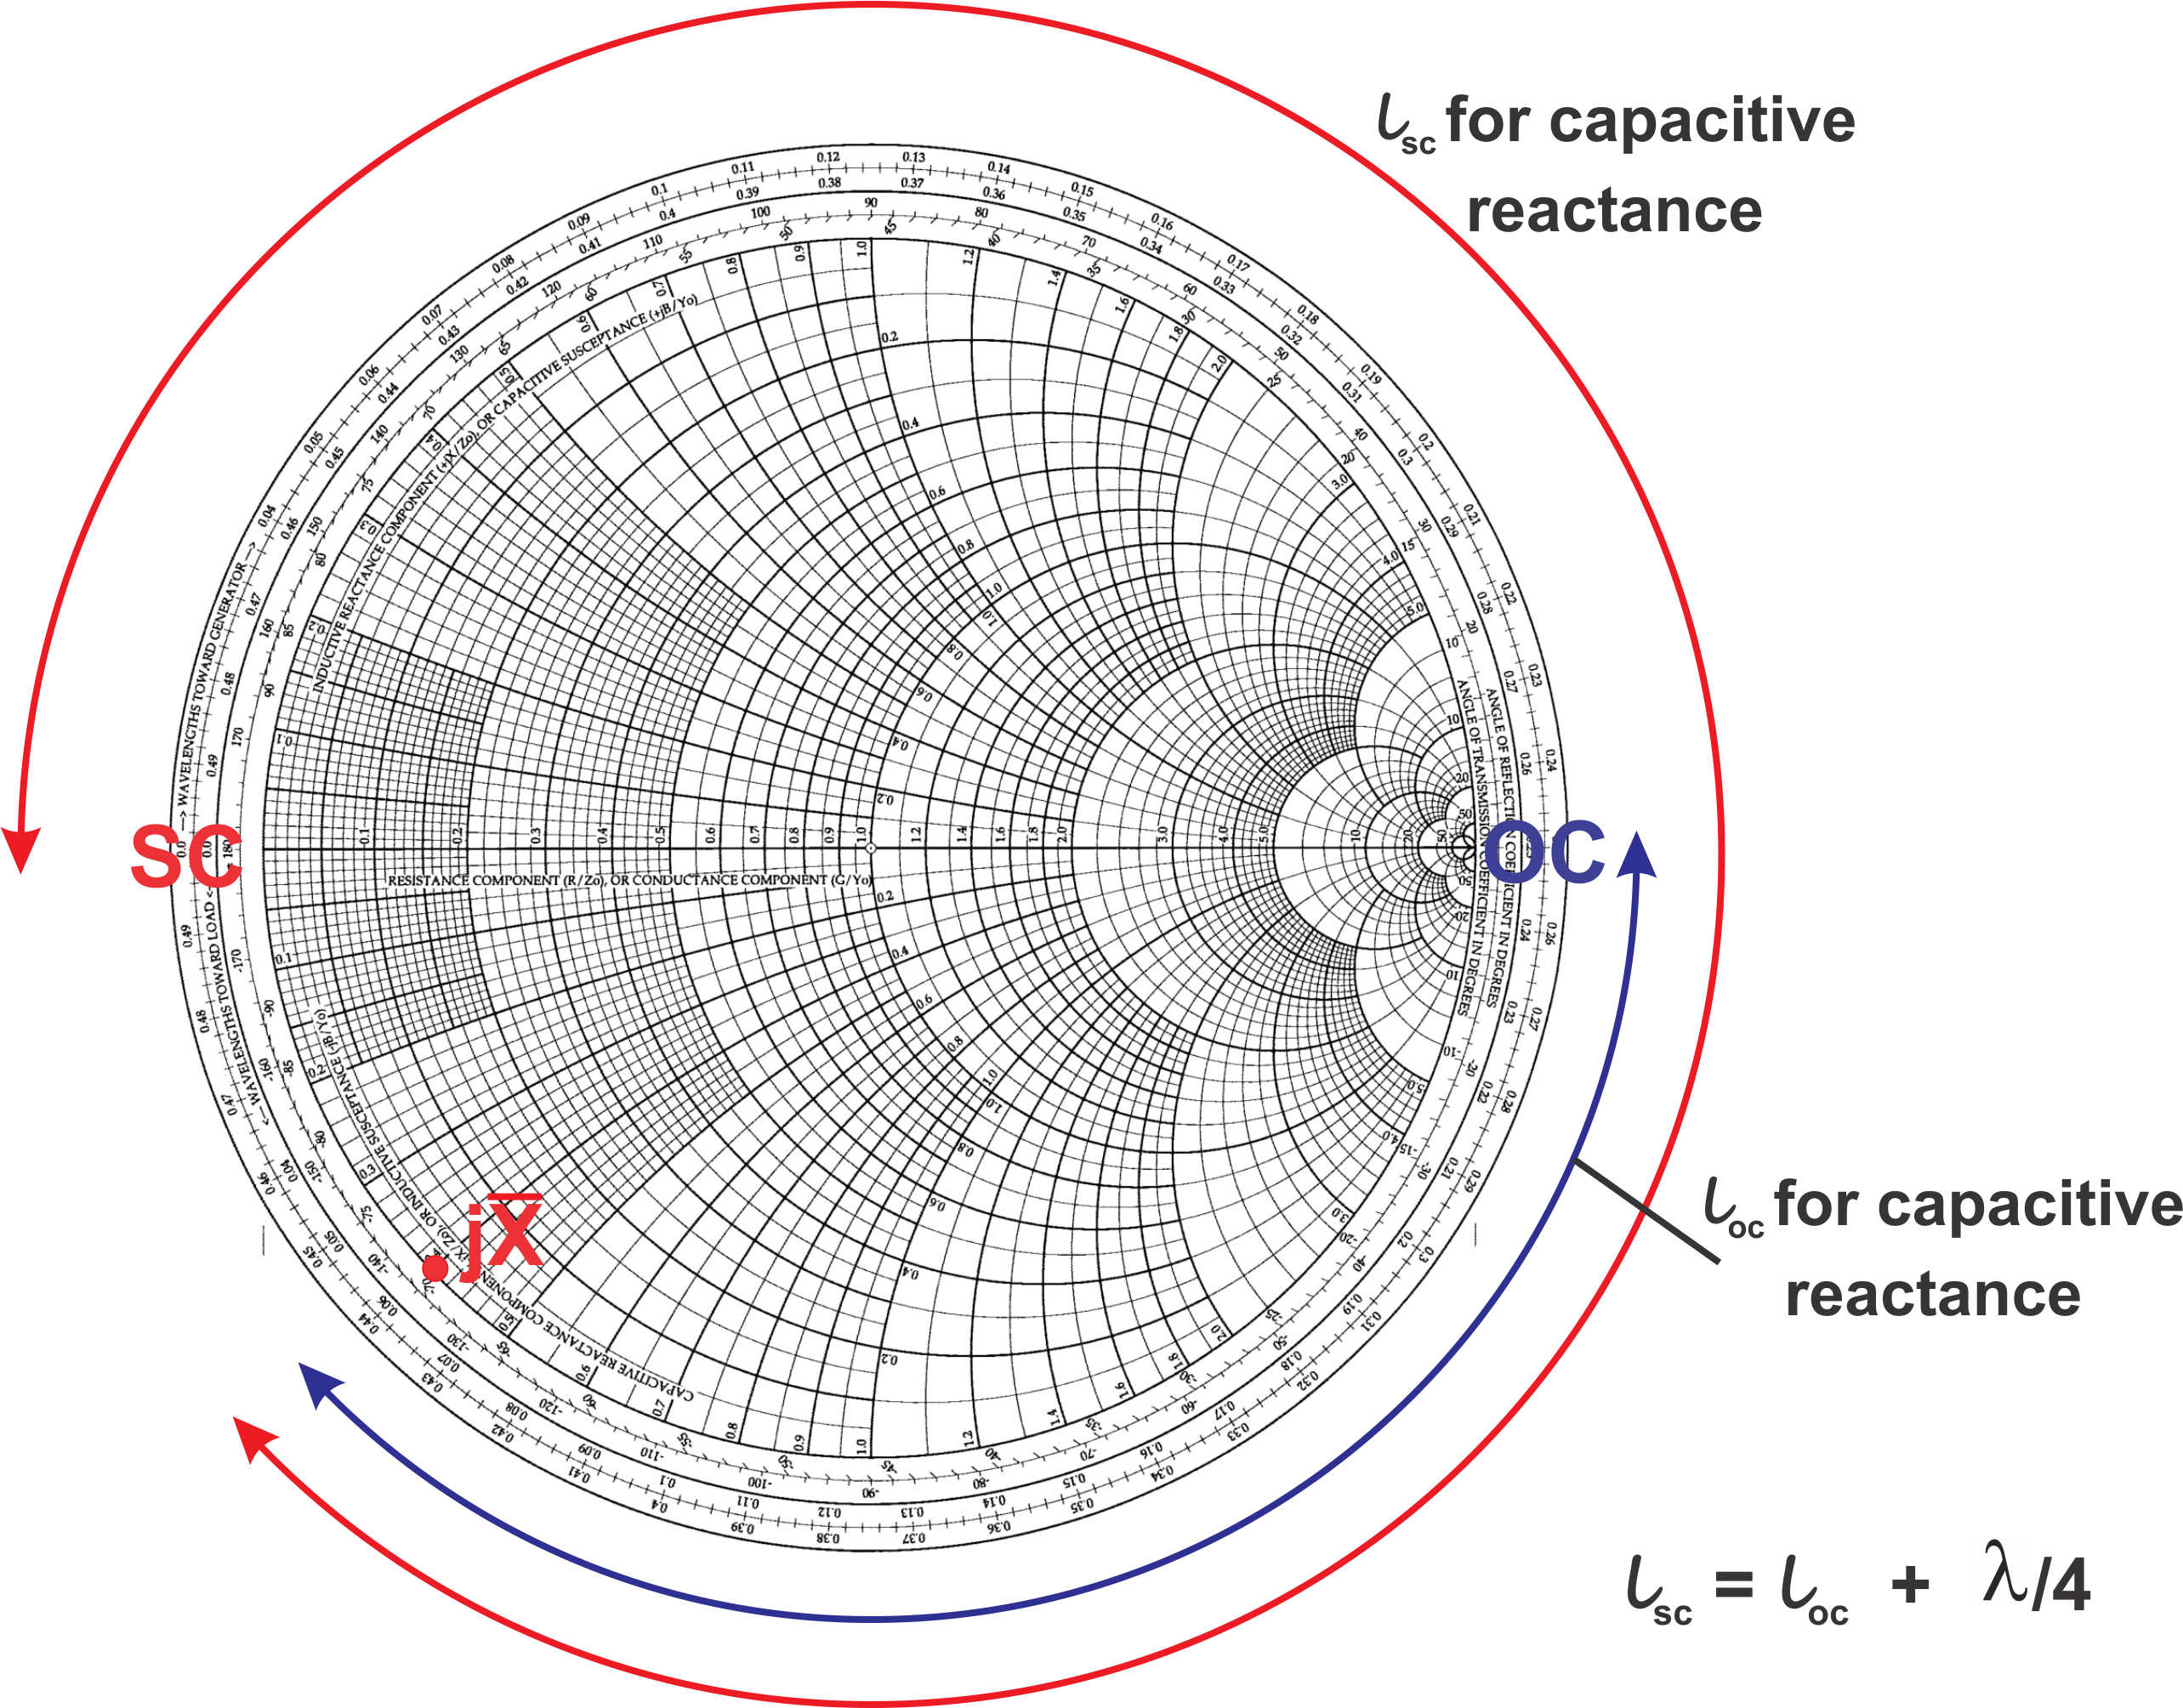
\includegraphics[scale=0.4]{./graphics/group10diagram8}
\caption{$ l_{SC} $ and $ l_{OC} $ for capacitive reactance on the Smith Chart}
\label{fig:group10diagram9}
\end{figure}

Hence if the length lies within 0 and $ \frac{\lambda}{4} $ for a short circuited line, we have inductive reactance while if the length lies from $ \frac{\lambda}{4} $ to $ \frac{\lambda}{2} $ we have capacitive reactance. Similarly for an open circuit line, if  the length lies within 0 to $ \frac{\lambda}{4} $, we have capacitive reactance and if it lies within $ \frac{\lambda}{4} $ to $ \frac{\lambda}{2} $ we have inductive reactance. It can be written explicitly in the figure~\ref{fig:group10diagram10}:
\begin{figure}[h]
\centering
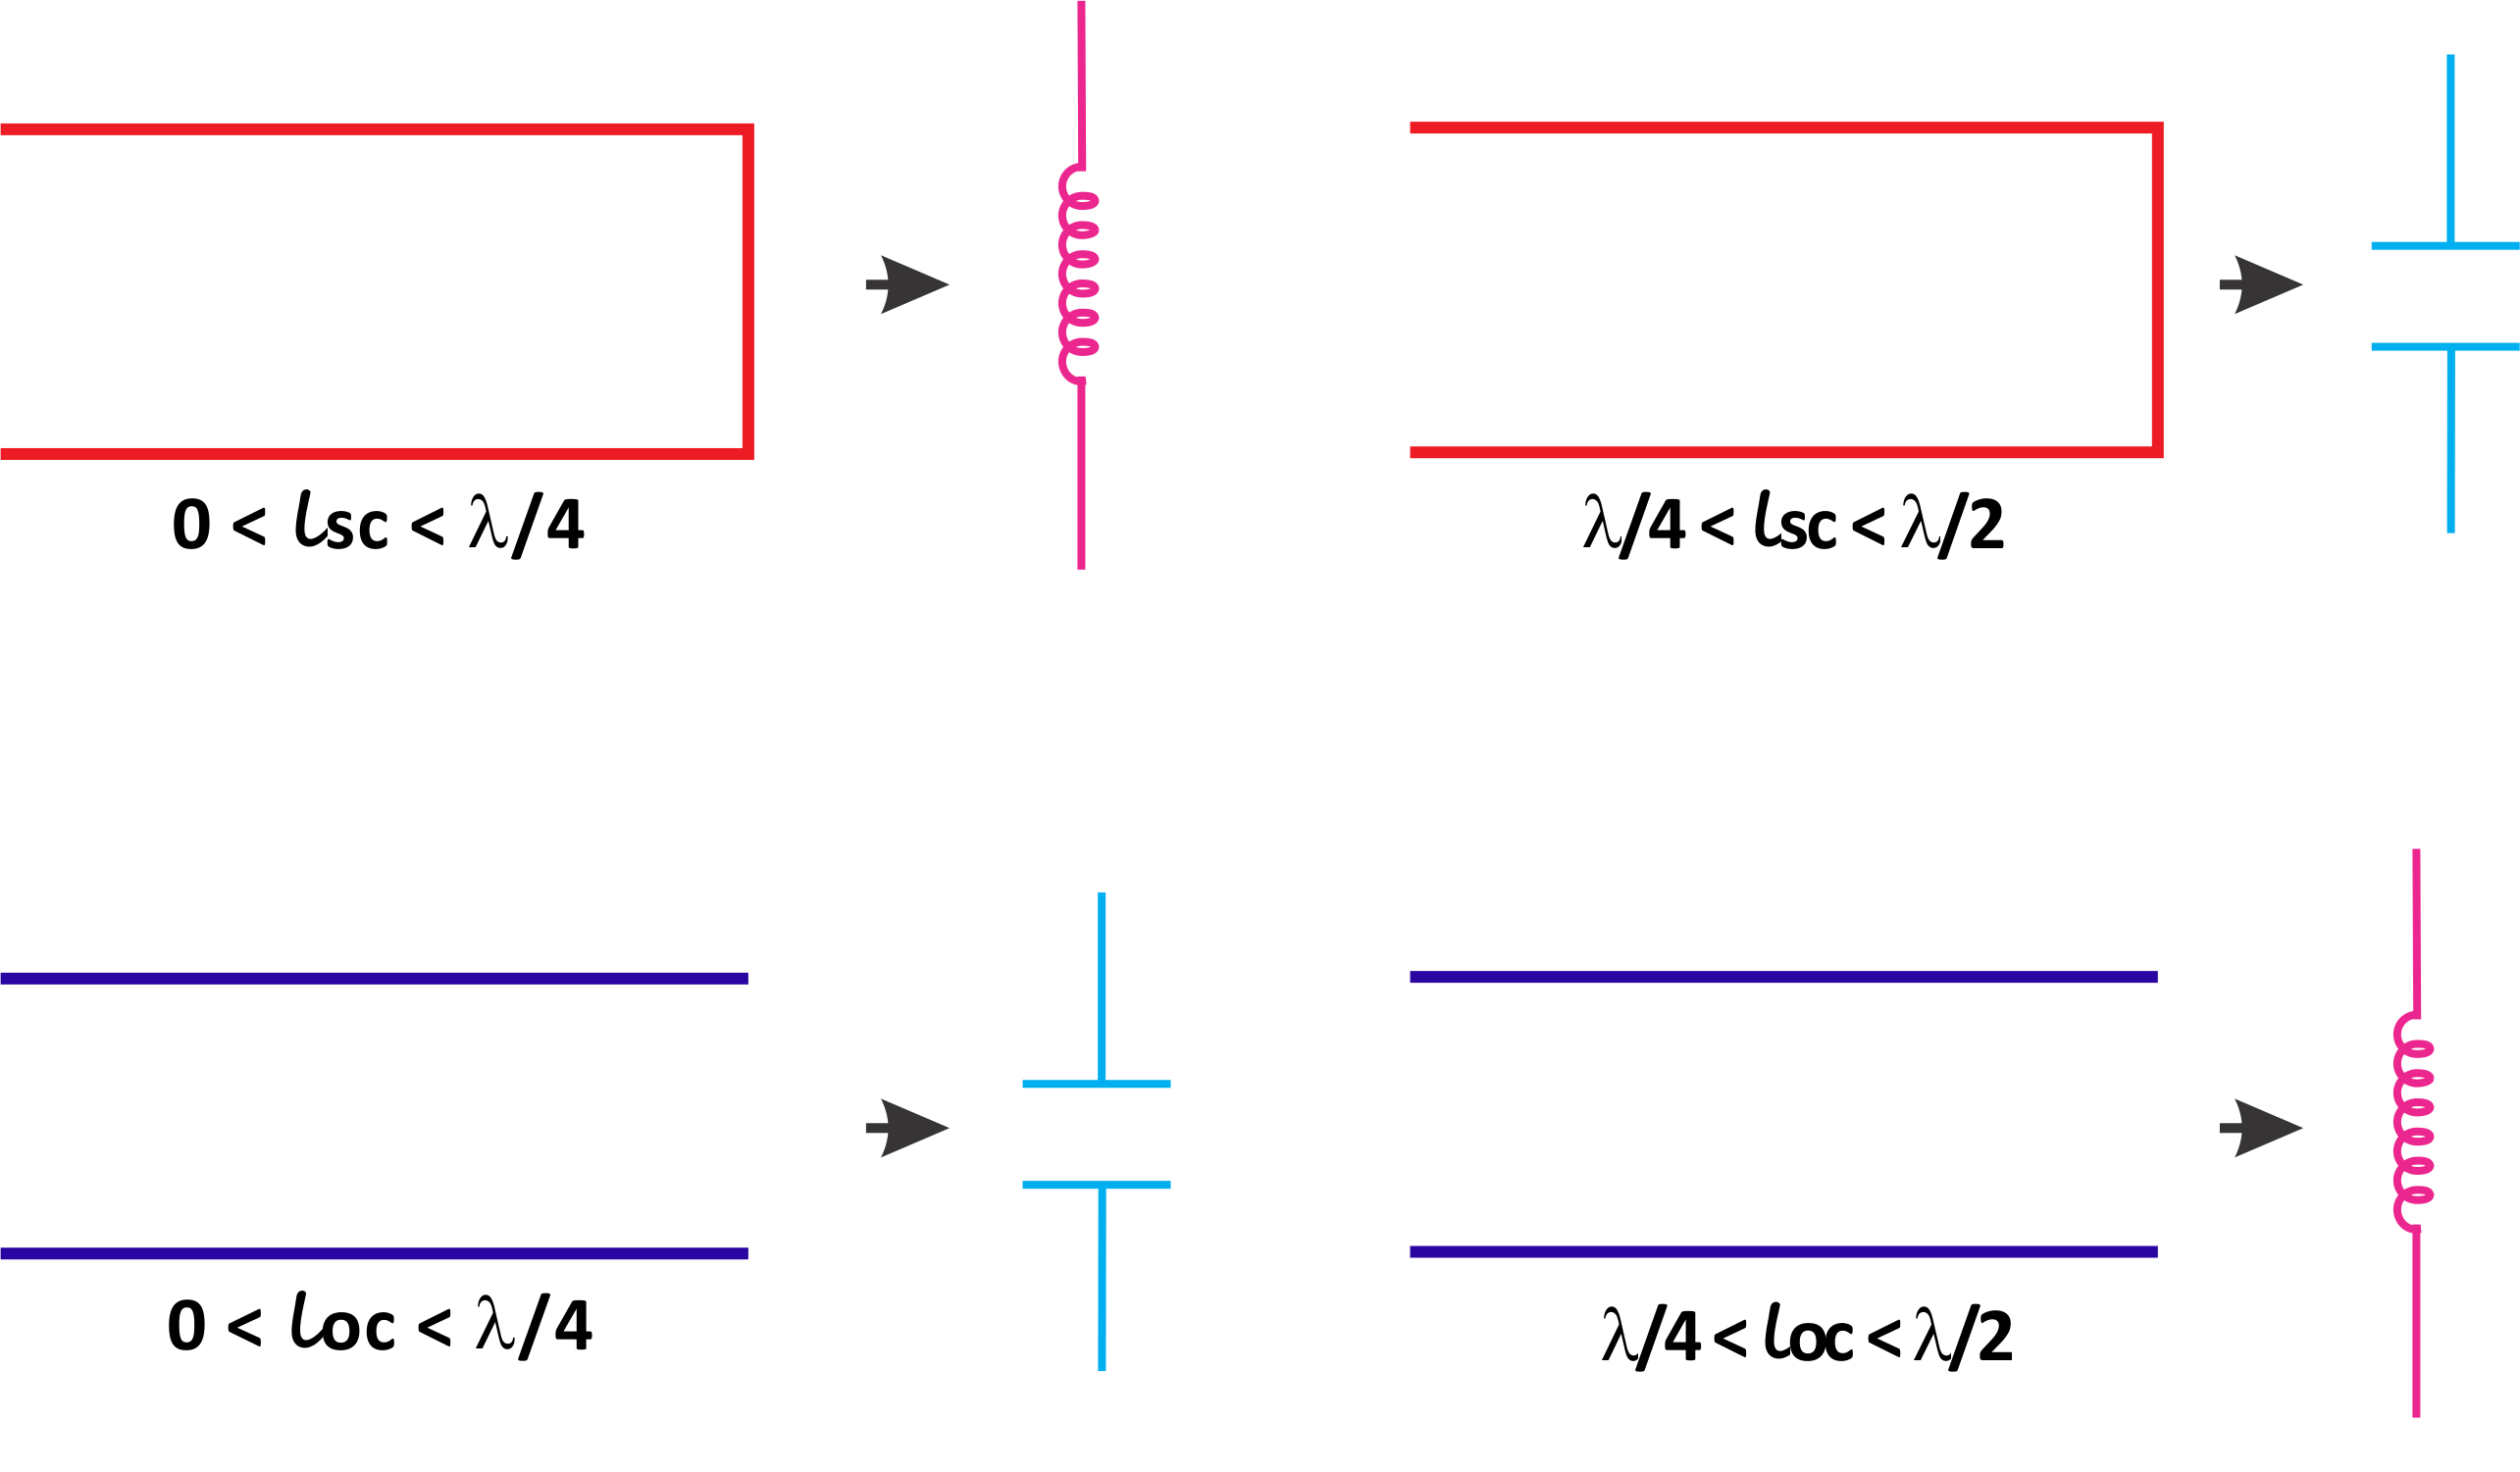
\includegraphics[width=1\linewidth]{./graphics/group10diagram9}
\caption{Nature of impedance for $ l_{SC} $ and $ l_{OC} $ after moving the different lengths}
\label{fig:group10diagram10}
\end{figure}

So any transection of a transmission line of size 0 to $ \frac{\lambda}{2} $ can realize any arbitrary value of capacitance and inductance at a particular frequency. We are not realizing a capacitor or inductor in actual sense, but we are realizing capacitive and inductive reactance.

\section{As a Resonant circuit}
At $ \frac{\lambda}{4} $ the behaviour of the line changes from $ X_{L} $ to $ X_{C} $ or $ X_{C} $ to $ X_{L} $. Such a behaviour is similar to the characteristics of resonance, that is, at $\frac{\lambda}{4}$  location, we have a characteristics that is more like resonance characteristics. Let us suppose we have a circuit, at resonant frequency\footnote{
Resonance frequency is a frequency point where the inductive reactance of the inductor becomes equal in value to the capacitive reactance of the capacitor $ X_{L} = X_{C} $
}, a part of the circuit has inductive behaviour while the other part has capacitive behaviour. 

So a transection of a transmission line may not only be used as a reactive element, it can also be used as a resonant LC circuit\footnote{
It consist of an inductor and capacitor connected together. It is used for generating signals at a particular frequency or picking out a signal at a particular frequency from a more complex signal
}. Now we see that suppose you take a line at $ \frac{\lambda}{4} $ to $ \frac{\lambda}{2} $, it will have a behaviour similar to the LC resonant circuit. It means that if we change the frequency for a given length of a transmission line, the impedance seen between the terminals of the line is going to change.
\begin{figure}[h]
\centering
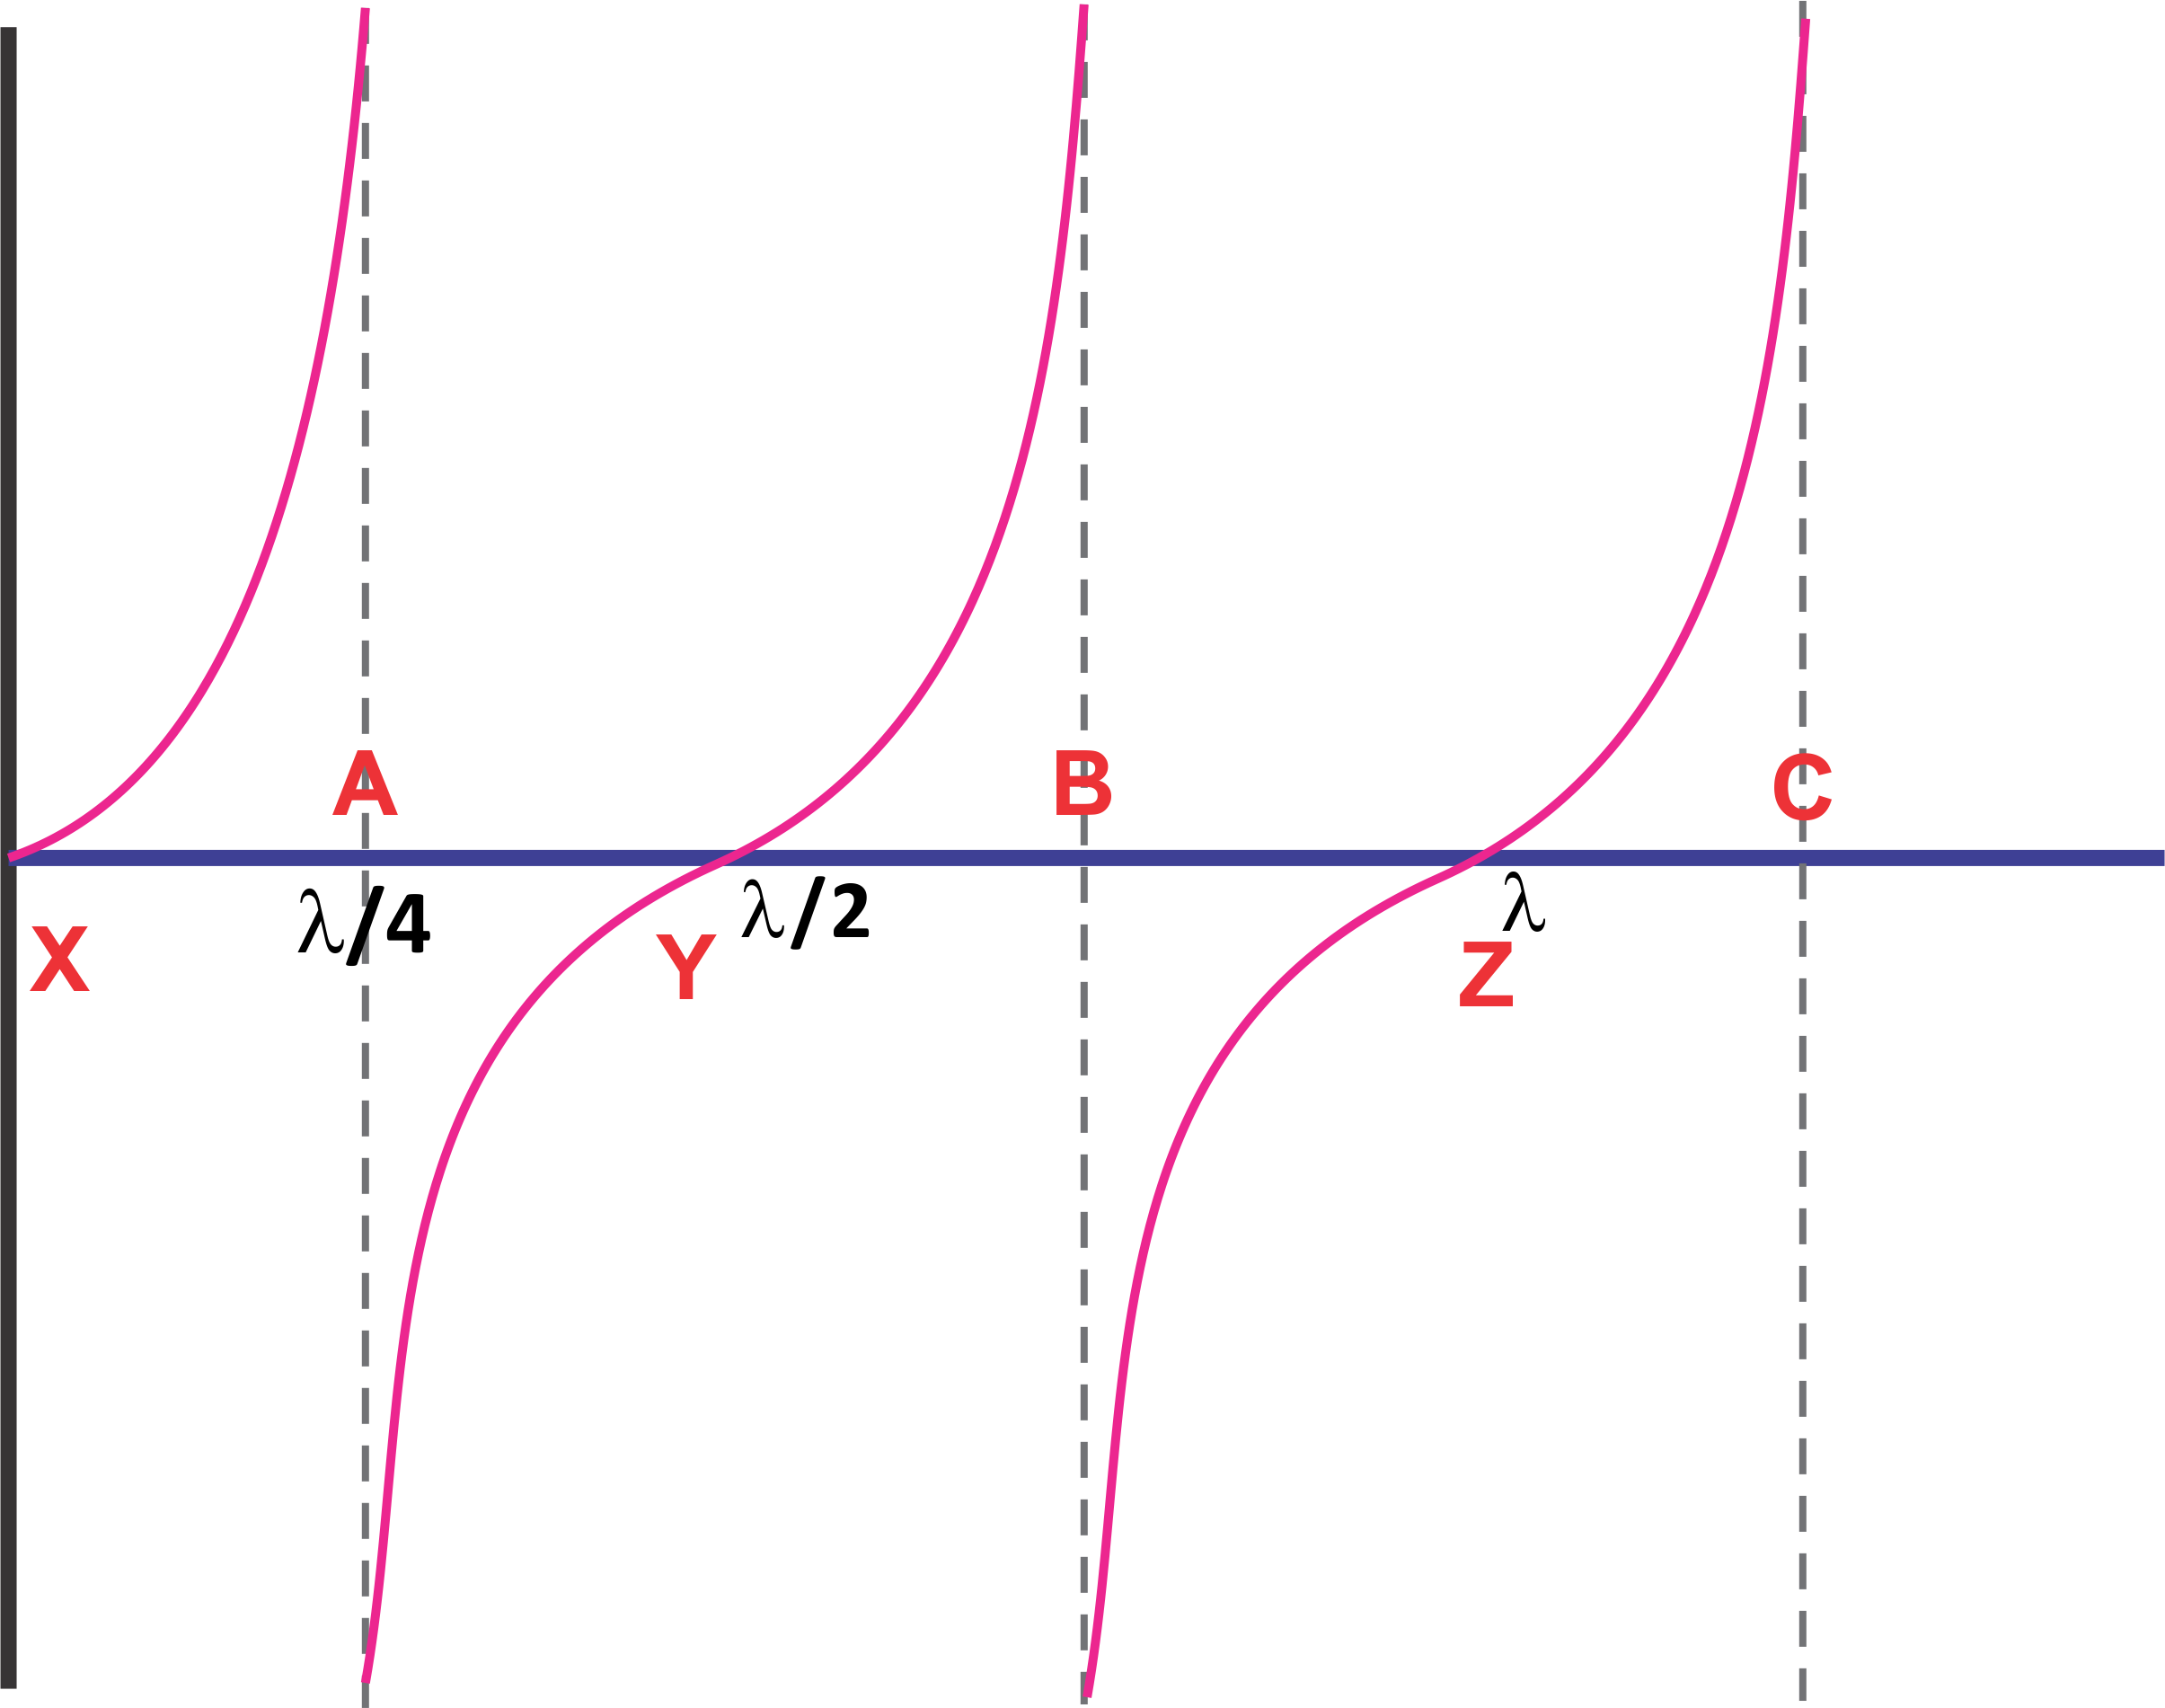
\includegraphics[width=0.7\linewidth]{./graphics/group10diagram10}
\caption{Resonance Characteristics for a short circuit end transmission line}
\label{fig:group10diagram11}
\end{figure}

For a short circuit whose length is $ \frac{\lambda}{2} $, the impedance is equal to zero since the impedance repeats every $\frac{\lambda}{2}$. At $ \frac{\lambda}{4} $ the line will be an open circuit and the impedance will be $\infty$. When the frequency is such that the length is zero (0) or $ \frac{\lambda}{2} $ or $ \lambda $ we get zero impedance (see figure~\ref{fig:group10diagram11}). However, if we go to the frequency for which the length is $ \frac{\lambda}{4} $, the impedance seen between the terminals of the lines is $\infty$ since it will appear like an open circuit.

So for a given frequency as we change the line length, when the line length is $ 0, \frac{\lambda}{2}, \lambda $ we see impedances at X, Y and Z. At frequency for which the length is $ \frac{\lambda}{4}, \frac{3\lambda}{4}, \frac{5\lambda}{4} $ we see impedance at A, B and C\footnote{
We are dealing with short circuit for this analysis
}. Starting from the short circuit (SC) point on the Smith Chart $ \frac{\lambda}{4} $, $ \frac{3\lambda}{4} $, $ \frac{5\lambda}{4} $ movement will correspond to a open circuit or $ \infty $ impedance,  hence A, B and C on the graph. Also, $ \frac{\lambda}{2} $, $ \lambda $, $ \frac{3\lambda}{2} $ will correspond to a SC point, which is the point we started from\footnote{
rRecall that a complete $ 2\pi $ movement correspond to $ \frac{\lambda}{2} $ on the Smith Chart
}. Hence in the frequency range close to X, Y and Z we have characteristics similar to that of a series LC circuit
at resonance (see figure~\ref{fig:group10diagram12}). However in the vicinity of A, B and C the behaviour is similar to that of a parallel LC circuit at resonance (see figure~\ref{fig:group10diagram13}). 
\begin{figure}[h]
\centering
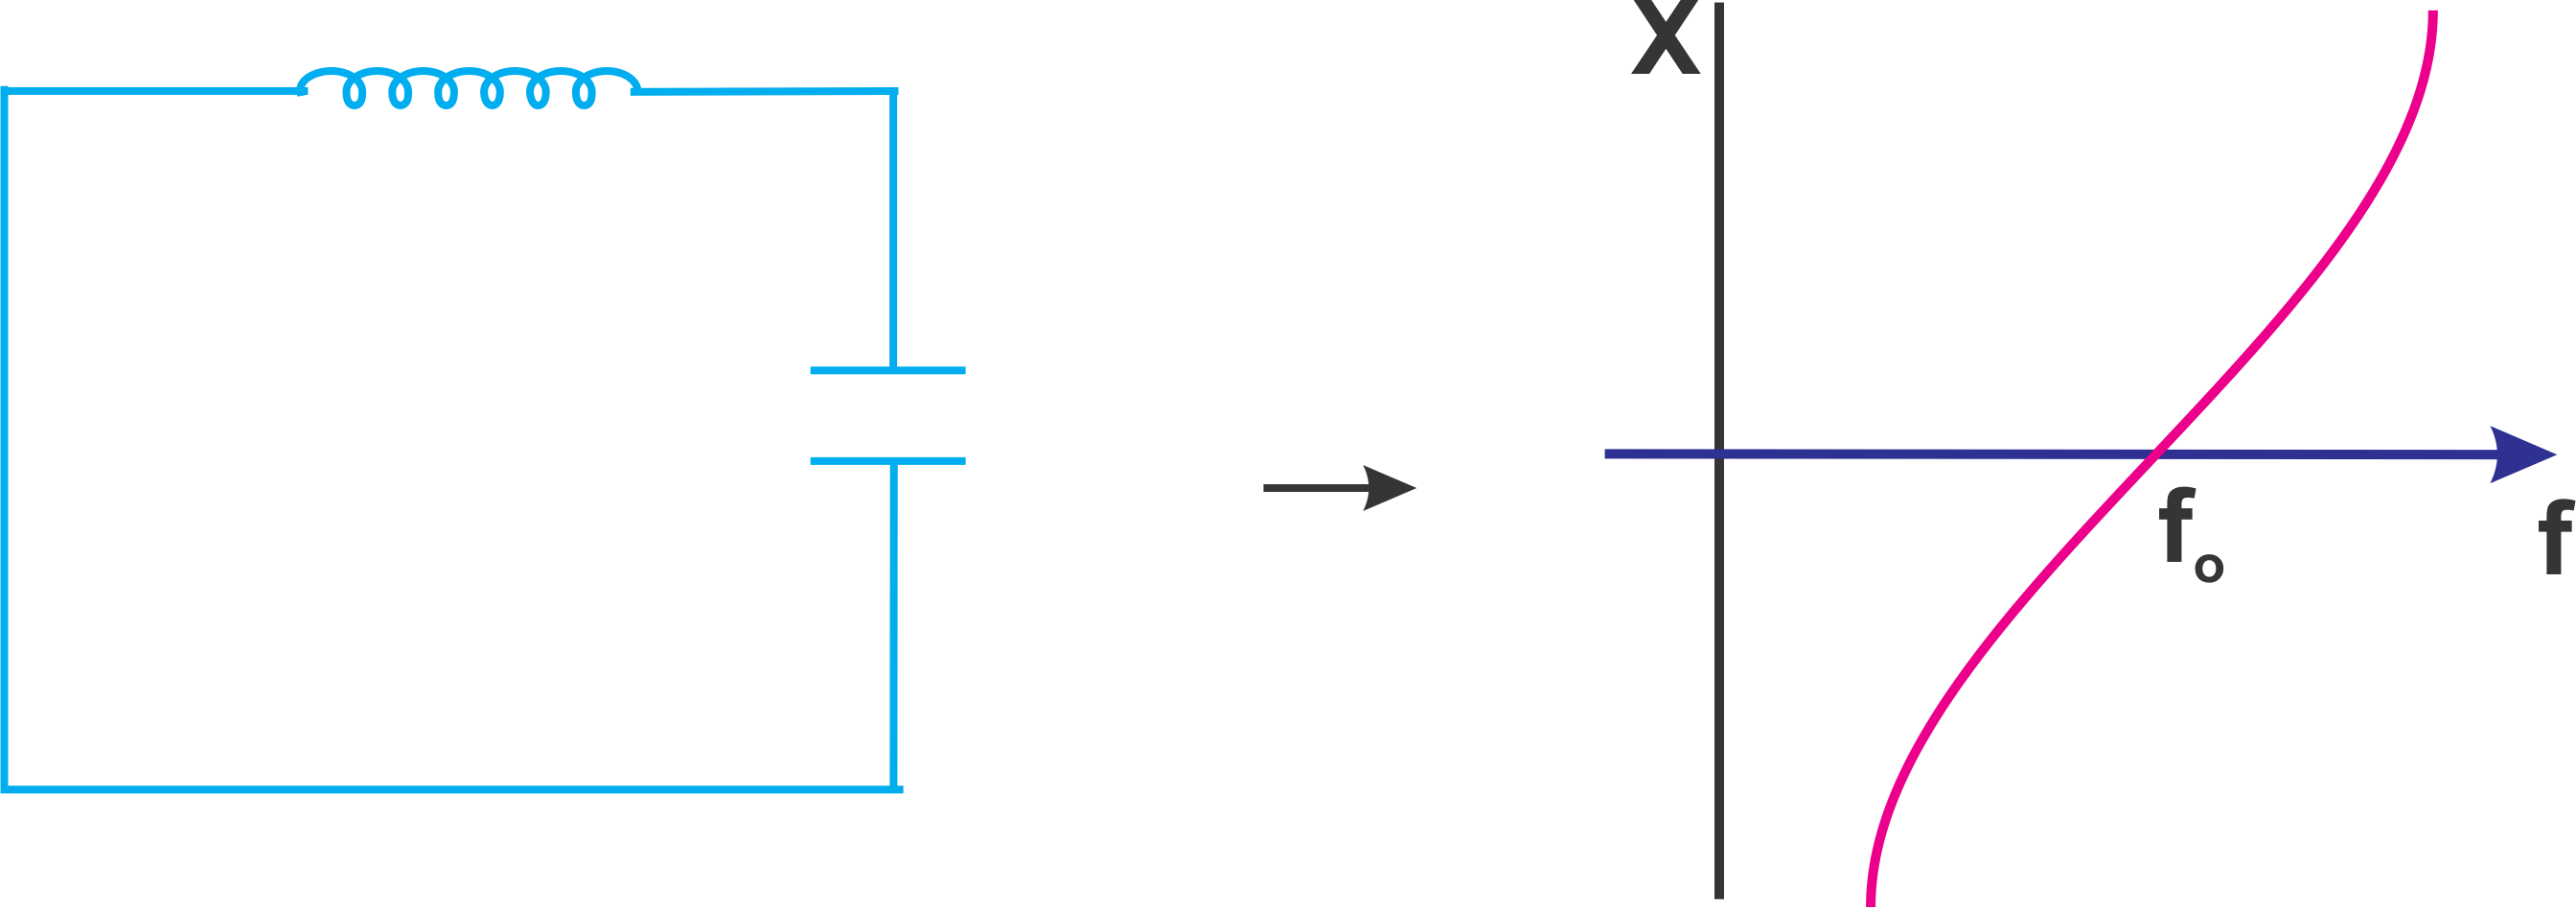
\includegraphics[width=1\linewidth]{./graphics/group10diagram11}
\caption{Series LC Circuit}
\label{fig:group10diagram12}
\end{figure}
\begin{figure}[h]
\centering
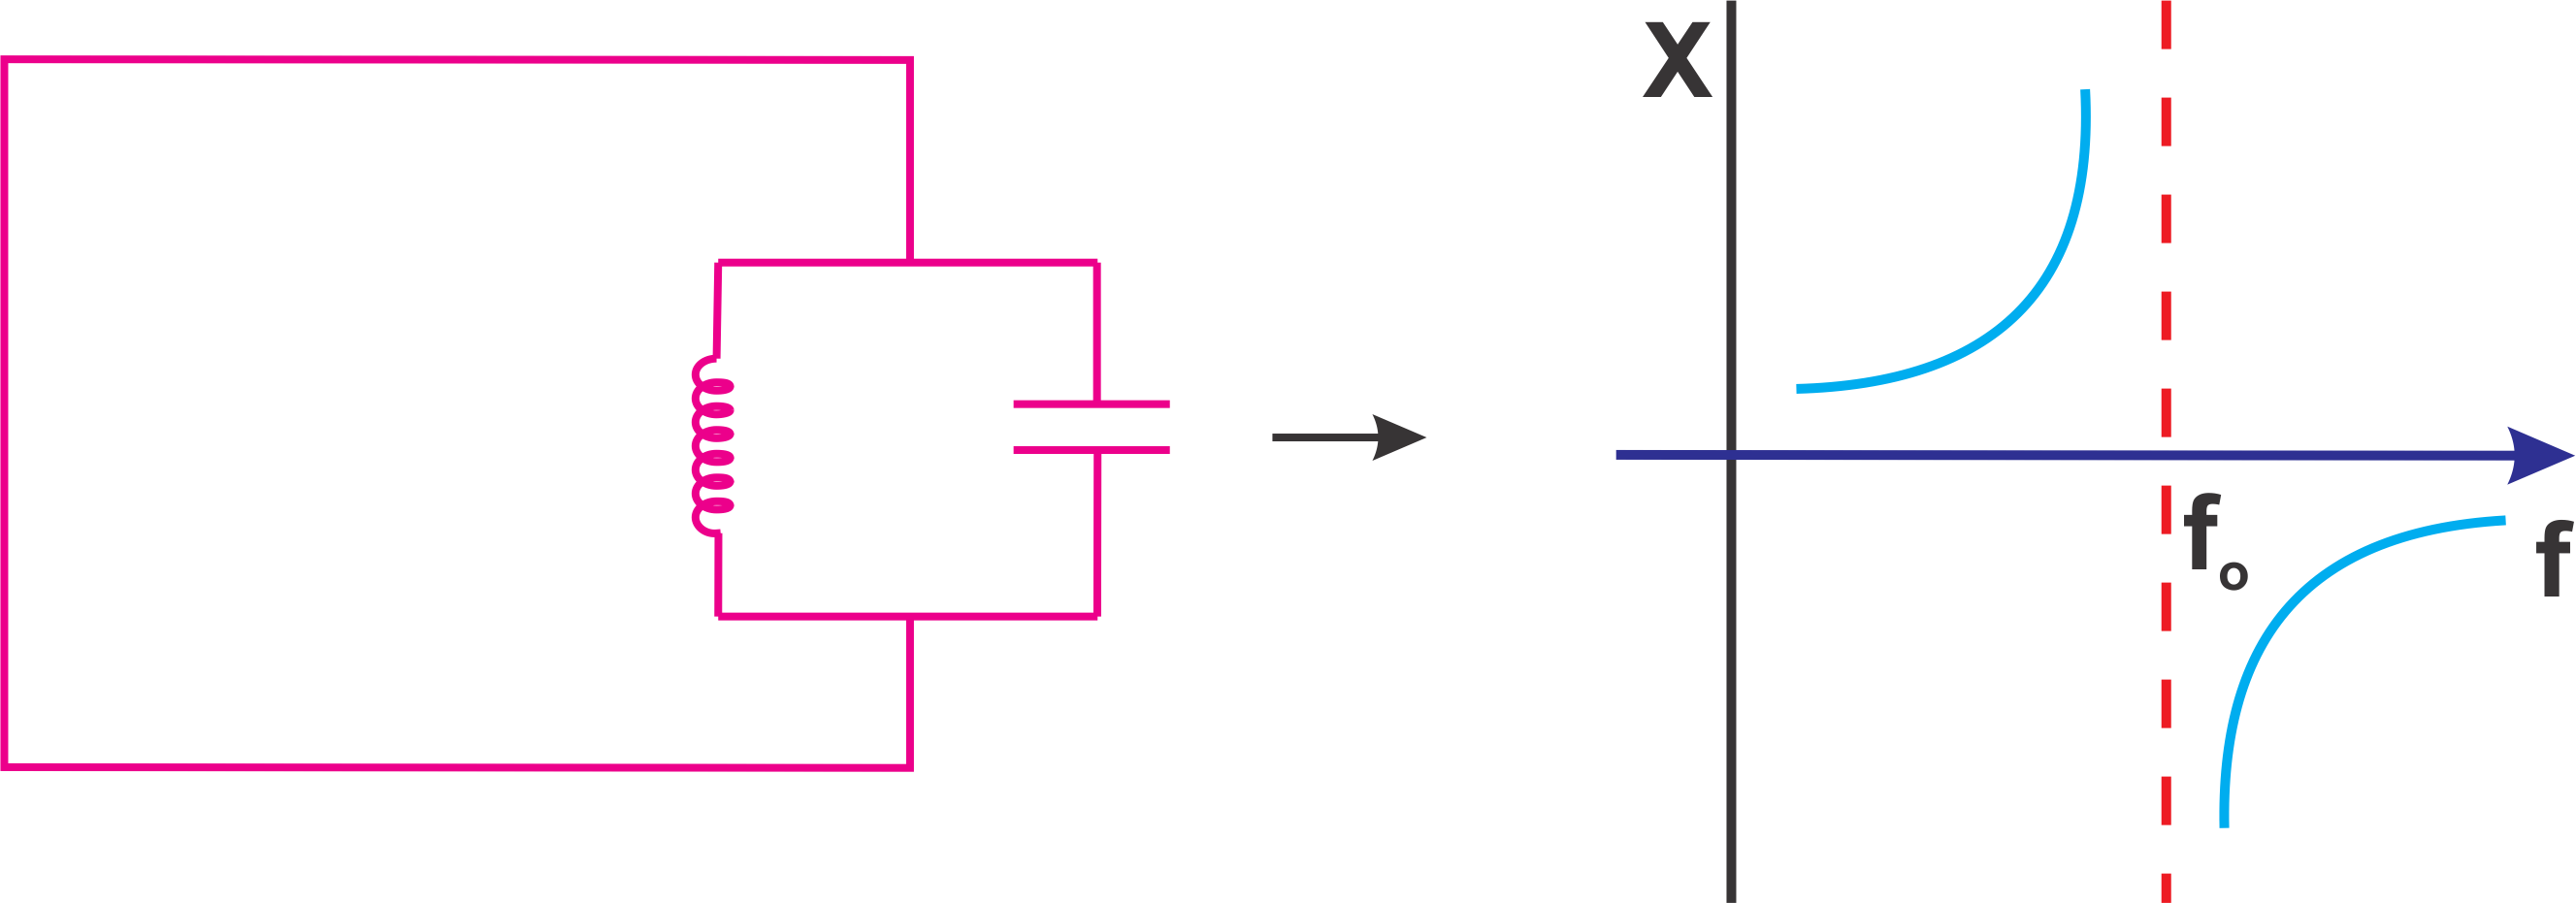
\includegraphics[width=1\linewidth]{./graphics/group10diagram12}
\caption{Parallel LC Circuit}
\label{fig:group10diagram13}
\end{figure}

\subsection{Resonance for Series LC Circuit}
From the characteristics of series LC circuit, we know that at resonance frequency, $X_L = X_C$. As frequency increases, then $ X_{L} > X_{C} $ then we have a positive $X$, and conversely, as frequency decreases, then $ X_{C} > X_{L} $ therefore we have negative $X$ (see figure~\ref{fig:group10diagram12}).

\subsection{Resonance for Parallel LC Circuit}
At resonance frequency, the equivalent impedance, $X$ is $\infty$ that is
\begin{align*}
\frac{1}{X} = \frac{1}{X_{C}} + \frac{1}{X_{L}} = 0
\end{align*}
At lower frequency, $ \frac{1}{X_{L}} $ is larger than $ \frac{1}{X_{C}} $. So $ X_{L} $ component dominates in the equivalent $X$. At higher frequencies, the $\frac{1}{X_C}$ is larger than $\frac{1}{X_L}$ (see figure~\ref{fig:group10diagram13}).

So a transmission line can behave like a series resonance circuit of a series LC circuit, and can behave like a parallel resonance circuit of a parallel LC circuits. For a given length of transmission line, those frequencies for which the length of the line tends to $ \frac{\lambda}{2} $ the line will behave like series resonance circuit. On the other hand for those frequencies for which the length of the line tends to $ \frac{\lambda}{4} $, the line behaves like a parallel resonance circuit. The analysis of transmission line as a resonant circuit was done for a short circuit end and as such the opposite observations will be made for an open circuit end transmission line.

For an open circuit whose length is $ \frac{\lambda}{2} $, the impedance is equal to infinity. At $ \frac{\lambda}{4} $ the line will be a short circuit and the impedance will be equal to zero. One side of that frequency will be capacitive that is, negative. So when the frequency is such that the length is zero (0) or $ \frac{\lambda}{2} $ or $ \lambda$ we get an impedance equal to infinity.
However, if we go to the frequency for which the length is $ \frac{\lambda}{4} $ , the impedance seen between the terminals of the lines is zero. So for a given frequency as we change the line length, when the line
length is $0, \frac{\lambda}{2}, \lambda $ we see impedances at A, B and C as shown in figure~\ref{fig:group10diagram15}. At frequency for which the length is $ \frac{\lambda}{4}, \frac{3\lambda}{4}, \frac{5\lambda}{4} $ we are at X, Y and Z.
\begin{figure}[h]
\centering
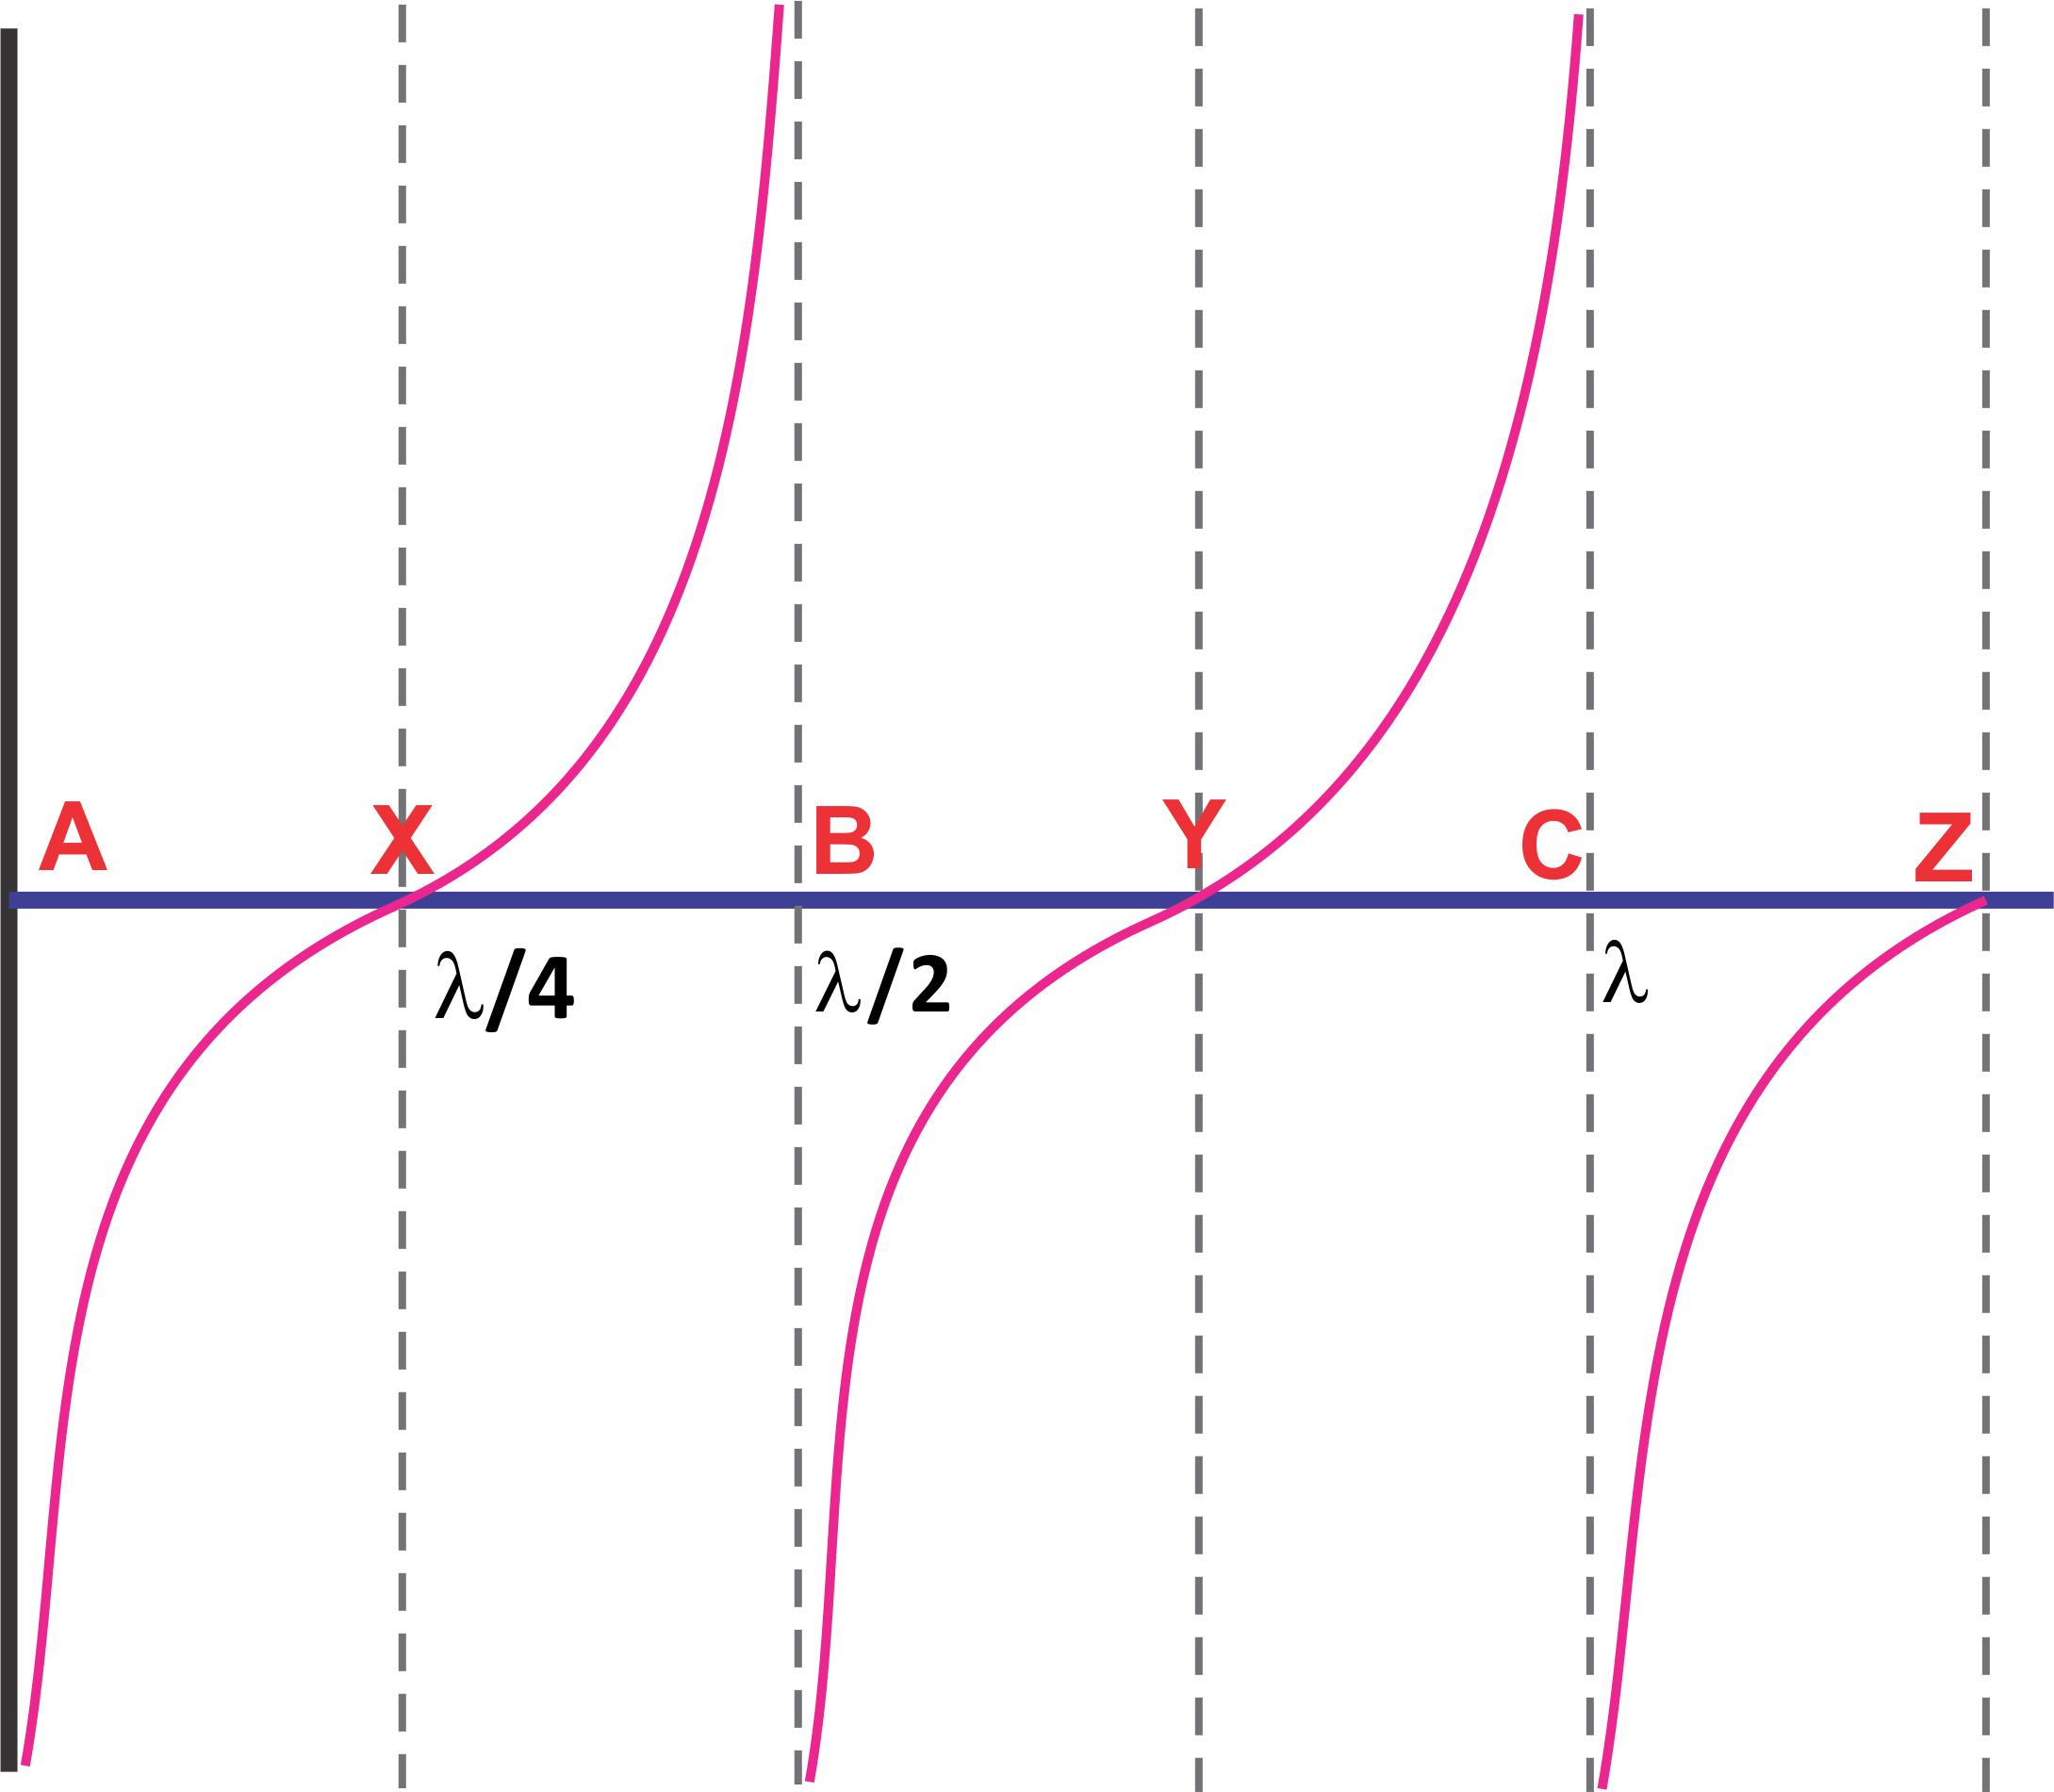
\includegraphics[width=.8\linewidth]{./graphics/group10diagram14}
\caption{Resonance Characteristics for an open circuit end transmission line}
\label{fig:group10diagram15}
\end{figure}

For open circuit line for length around $ \frac{\lambda}{2} $, the line will behave like a parallel resonant circuit because the input impedance will be at infinity. At about $ \frac{\lambda}{4} $, the line is like a short circuit and so behaves like a series resonant circuit. If the length of the line is $ \frac{\lambda}{2} $ the line will behave like a parallel resonant circuit.
So depending upon whether short circuit line or open circuit line is used, the series or parallel resonance circuit can be realized at different frequencies. So invariably, at high frequencies, the transmission line can be used for realizing circuit elements and series or parallel resonance circuits.

\subsection{Quality Factor of a resonant transmission line circuit}
So \emph{what is the quality factor of the resonant circuit?} By definition, quality factor is related to the losses of the circuit (the higher the loss, the smaller the quality factor). So whenever we have a reactive element like inductor or capacitor, the losses in these elements characterize the quality factor. Quality Factor is a parameter that describes how under-damped an oscillator or resonator is and characterizes a resonator's bandwidth relative to its center frequency. It is a dimensionless quantity. It is a measure of the quality of a resonant circuit. 

If we are dealing with lossless transmission line, then the quality factor for the resonance circuits should be infinite. There is no loss, however in practice, there is always a small loss in the transmission line. Hence we will shift our analysis from lossless transmission line to low-loss transmission line. This analysis will be treated in the next.
